% Main document
% ===========================================================================
% This is part of the document "Project documentation template".
% Authors: brd3, kaa1
%
%---------------------------------------------------------------------------
\documentclass[
	a4paper,				% paper format
	10pt,					% fontsize
%	twoside,				% double-sided
	openright,				% begin new chapter on right side
	notitlepage,				% use no standard title page
	parskip=half,				% set paragraph skip to half of a line
]{scrreprt}					% KOMA-script report
%---------------------------------------------------------------------------

\raggedbottom
%\KOMAoptions{cleardoublepage=plain}		% Add header and footer on blank pages


% Load Standard Packages:
%---------------------------------------------------------------------------
\usepackage[standard-baselineskips]{cmbright}

\usepackage[ngerman]{babel}			% german hyphenation
%\usepackage[latin1]{inputenc}  		% Unix/Linux - load extended character set (ISO 8859-1)
%\usepackage[ansinew]{inputenc}  		% Windows - load extended character set (ISO 8859-1)
\usepackage[utf8]{inputenc}
\usepackage[T1]{fontenc}			% hyphenation of words with ä,ö and ü
\usepackage{textcomp}				% additional symbols
\usepackage{ae}					% better resolution of Type1-Fonts 
\usepackage{fancyhdr}				% simple manipulation of header and footer 
\usepackage{etoolbox}				% color manipulation of header and footer
\usepackage{graphicx}                   	% integration of images
\usepackage{float}				% floating objects
\usepackage{caption}				% for captions of figures and tables
\usepackage{booktabs}				% package for nicer tables
\usepackage{tocvsec2}				% provides means of controlling the sectional numbering
%---------------------------------------------------------------------------

% Packages ausserhalb "BFH Standard"
%---------------------------------------------------------------------------
\usepackage[
	backend=biber,
	style=numeric,
	sorting=anyt
]{biblatex}
\addbibresource{datenbanken/references.bib}

\usepackage[toc, acronym]{glossaries}
\usepackage{glossaries}
\usepackage{keystroke}
%---------------------------------------------------------------------------

% Load Math Packages
%---------------------------------------------------------------------------
\usepackage{amsmath}                    	% various features to facilitate writing math formulas
\usepackage{amsthm}                       	% enhanced version of latex's newtheorem
\usepackage{amsfonts}                      	% set of miscellaneous TeX fonts that augment the standard CM
\usepackage{amssymb}				% mathematical special characters
\usepackage{exscale}				% mathematical size corresponds to textsize
%---------------------------------------------------------------------------

% Package to facilitate placement of boxes at absolute positions
%---------------------------------------------------------------------------
\usepackage[absolute]{textpos}
\setlength{\TPHorizModule}{1mm}
\setlength{\TPVertModule}{1mm}
%---------------------------------------------------------------------------					
			
% Definition of Colors
%---------------------------------------------------------------------------
\RequirePackage{color}                          % Color (not xcolor!)
\definecolor{linkblue}{rgb}{0,0,0.8}            % Standard
\definecolor{darkblue}{rgb}{0,0.08,0.45}        % Dark blue
\definecolor{bfhgrey}{rgb}{0.41,0.49,0.57}      % BFH grey
%\definecolor{linkcolor}{rgb}{0,0,0.8}     	% Blue for the web- and cd-version!
\definecolor{linkcolor}{rgb}{0,0,0}        	% Black for the print-version!

%---------------------------------------------------------------------------

% Listings Packages ausserhalb "BFH Standard"
%---------------------------------------------------------------------------
\newcommand{\titel}		{LIDAR Einbindung für den Robocup}
\newcommand{\versionnumber}	{abcdef}
\newcommand{\versiondate}	{\today}
\newcommand{\datum}		{\today}
\newcommand{\studiengang}	{Informatik, berufsbegleitend}
\newcommand{\autor}		{Marco Kilchhofer}
\newcommand{\betreuer}		{Dr. Reto Koenig, \acrshort{bfh}}
\newcommand{\auftraggeber}	{Alain Rohr, \acrshort{hftm} / Dr. Reto Koenig, \acrshort{bfh}}
\newcommand{\experte}		{Dr. Joachim Wolfgang Kaltz}

\usepackage{listings}

\definecolor{listing-background}{rgb}{1.0,0.98,0.804}
\definecolor{listing-string}{rgb}{0,0.39,0}
\definecolor{listing-comment}{rgb}{0.65,0.65,0.65}
\definecolor{asparagus}{rgb}{0.53, 0.66, 0.42}
\definecolor{ao(english)}{rgb}{0.0, 0.5, 0.0}
\definecolor{verbatimcolor}{gray}{0.93}
\lstset{
	basicstyle=\small\ttfamily,
	language=Java,
	captionpos=b,
	numberstyle=\tiny,
	numbers=left,
	columns=fullflexible,
	frame=lines,
	framexleftmargin=0.5em,
	framexrightmargin=0.5em,
	backgroundcolor=\color{listing-background},
	keywordstyle=\color{blue},
	stringstyle=\color{listing-string},
	commentstyle=\color{listing-comment},
	showstringspaces=false,
	breaklines=true,
	breakatwhitespace=true
}
\lstdefinelanguage{none}{
	identifierstyle=
}

\definecolor{Maroon}{rgb}{0.0, 0.5, 0.0}
\definecolor{DarkOliveGreen}{rgb}{0.53, 0.66, 0.42}
\lstdefinelanguage{XML}
{
	morestring=[b]",
	morestring=[s]{>}{<},
	morecomment=[s]{<?}{?>},
	morecomment=[s]{<!--}{-->},
	stringstyle=\color{listing-string},
	identifierstyle=\color{darkblue},
	keywordstyle=\color{blue},
	morekeywords={xmlns,groupId,artifactId,packaging,classifier,version,type}
}

\newcommand{\ctexttt}[1]{\colorbox{verbatimcolor}{\texttt{#1}}}

%---------------------------------------------------------------------------

% Packages ausserhalb "BFH Standard" (Zitat)
%---------------------------------------------------------------------------
% for adjustwidth environment
\usepackage[strict]{changepage}

% for formal definitions
\usepackage{framed}

% environment derived from framed.sty: see leftbar environment definition
\definecolor{formalshade}{rgb}{0.95,0.95,1}

\newenvironment{formal}{%
  \def\FrameCommand{%
    \hspace{1pt}%
    {\color{darkblue}\vrule width 2pt}%
    {\color{formalshade}\vrule width 4pt}%
    \colorbox{formalshade}%
  }%
  \MakeFramed{\advance\hsize-\width\FrameRestore}%
  \noindent\hspace{-4.55pt}% disable indenting first paragraph
  \begin{adjustwidth}{}{7pt}%
  \vspace{2pt}\vspace{2pt}%
}
{%
  \vspace{2pt}\end{adjustwidth}\endMakeFramed%
}


%---------------------------------------------------------------------------

% Hyperref Package (Create links in a pdf)
%---------------------------------------------------------------------------
\usepackage[
	pdftex,ngerman,bookmarks,plainpages=false,pdfpagelabels,
	backref={false},			% No index backreference
	colorlinks={true},			% Color links in a PDF
	hypertexnames={true},			% no failures "same page(i)"
	bookmarksopen={true},			% opens the bar on the left side
	bookmarksopenlevel={0},		% depth of opened bookmarks
	pdftitle={\titel},% PDF-property
	pdfauthor={\autor},			% PDF-property
	pdfsubject={\ArtDerArbeit},		% PDF-property
	pdfkeywords={\ArtDerArbeit, HFTM, BFH, kilcm1, 2018},
	linkcolor={linkcolor},		% Color of Links
	citecolor={linkcolor},		% Color of Cite-Links
	urlcolor={linkcolor},			% Color of URLs
]{hyperref}
%---------------------------------------------------------------------------

% Set up page dimension
%---------------------------------------------------------------------------
\usepackage{geometry}
\geometry{
	a4paper,
	left=28mm,
	right=15mm,
	top=30mm,
	headheight=20mm,
	headsep=10mm,
	textheight=242mm,
	footskip=15mm
}
%---------------------------------------------------------------------------

% Makeindex Package
%---------------------------------------------------------------------------
\usepackage{makeidx}                       	% To produce index
\makeindex					% Index-Initialisation
%---------------------------------------------------------------------------

% Glossary Package
%---------------------------------------------------------------------------
% the glossaries package uses makeindex
% if you use TeXnicCenter do the following steps:
%  - Goto "Ausgabeprofile definieren" (ctrl + F7)
%  - Select the profile "LaTeX => PDF"
%  - Add in register "Nachbearbeitung" a new "Postprozessoren" point named Glossar
%  - Select makeindex.exe in the field "Anwendung" ( ..\MiKTeX x.x\miktex\bin\makeindex.exe )
%  - Add this [ -s "%tm.ist" -t "%tm.glg" -o "%tm.gls" "%tm.glo" ] in the field "Argumente"
%
% for futher informations go to http://ewus.de/tipp-1029.html
%---------------------------------------------------------------------------
%\usepackage[nonumberlist]{glossaries}
%% Glossar
\newglossaryentry{contract}{
	name={Contract},
	description={Die Vereinbarung / der Vertrag der Schnittstelle zwischen Services und Servants.},
	plural={contracts}
}
\newglossaryentry{description}{
	name={Description},
	description={Description-Topic eines Services, für API-Dokumentation},
}
\newglossaryentry{event}{
	name={Event},
	description={Event-Topic eines Services, beispielsweise für Messwerte},
	plural={Events}
}
\newglossaryentry{intent}{
	name={Intent},
	description={Befehls-Topic eines Services, zum Absetzen von Steuerungsbefehlen an den Service},
	plural={Intents}
}
\newglossaryentry{payload}{
	name={Payload},
	description={Payload bezeichnet in MQTT die eigentliche Nachricht, also der Inhalt},
	plural={Payload}
}
\newglossaryentry{servant}{
	name={Servant},
	description={},
	plural={Servants}
}
\newglossaryentry{service}{
	name={Service},
	description={},
	plural={Services}
}
\newglossaryentry{status}{
	name={Status},
	description={Status-Topic eines Services, beispielsweise für Zustände und statische Informationen},
	plural={Stati}
}
\newglossaryentry{topic}{
	name={Topic},
	description={Topic bezeichnet in MQTT den Pfad unter welchem eine Nachricht veröffentlicht (published) wird},
	plural={Topics}
}
\newglossaryentry{unit}{
	name={Unit},
	description={eine Instanz eines Services},
	plural={Units}
}

% Glossar
\newglossaryentry{contract}{
	name={Contract},
	description={Die Vereinbarung / der Vertrag der Schnittstelle zwischen Services und Servants.},
	plural={contracts}
}
\newglossaryentry{description}{
	name={Description},
	description={Description-Topic eines Services, für API-Dokumentation},
}
\newglossaryentry{event}{
	name={Event},
	description={Event-Topic eines Services, beispielsweise für Messwerte},
	plural={Events}
}
\newglossaryentry{intent}{
	name={Intent},
	description={Befehls-Topic eines Services, zum Absetzen von Steuerungsbefehlen an den Service},
	plural={Intents}
}
\newglossaryentry{payload}{
	name={Payload},
	description={Payload bezeichnet in MQTT die eigentliche Nachricht, also der Inhalt},
	plural={Payload}
}
\newglossaryentry{servant}{
	name={Servant},
	description={},
	plural={Servants}
}
\newglossaryentry{service}{
	name={Service},
	description={},
	plural={Services}
}
\newglossaryentry{status}{
	name={Status},
	description={Status-Topic eines Services, beispielsweise für Zustände und statische Informationen},
	plural={Stati}
}
\newglossaryentry{topic}{
	name={Topic},
	description={Topic bezeichnet in MQTT den Pfad unter welchem eine Nachricht veröffentlicht (published) wird},
	plural={Topics}
}
\newglossaryentry{unit}{
	name={Unit},
	description={eine Instanz eines Services},
	plural={Units}
}

% Abkürzungen
\newacronym{api}   {API}   {Application Programming Interface, Programmierschnittstelle}
\newacronym{bfh}   {BFH}   {Berner Fachhochschule}
\newacronym{hftm}  {HFTM}  {Höhere Fachschule für Technik Mittelland}
\newacronym{lidar} {Lidar} {light detection and ranging}
\newacronym{mqtt}  {MQTT}  {Message Queuing Telemetry Transport}
\newacronym{yaml}  {YAML}  {YAML Ain’t Markup Language}
\newacronym{ros}   {ROS}   {Robot Operating System}

\makeglossaries
%---------------------------------------------------------------------------

% Intro:
%---------------------------------------------------------------------------
\begin{document}				% Start Document
\settocdepth{section}				% Set depth of toc
\pagenumbering{roman}														
%---------------------------------------------------------------------------

%\input{vorspann/titel}				% Titel der Arbeit aus Datei titel.tex lesen
%\input{vorspann/version}			% Versionsnummer und -datum aus Datei version.tex lesen

% Set up header and footer
%---------------------------------------------------------------------------
\makeatletter
\patchcmd{\@fancyhead}{\rlap}{\color{bfhgrey}\rlap}{}{}		% new color of header
\patchcmd{\@fancyfoot}{\rlap}{\color{bfhgrey}\rlap}{}{}		% new color of footer
\makeatother

\fancyhf{}						% clean all fields
\fancypagestyle{plain}{				% new definition of plain style	
%	\fancyfoot[OR,EL]{\footnotesize \thepage} 	% footer right part --> page number
%	\fancyfoot[OL,ER]{\footnotesize \titel, Version \versionnumber, \versiondate}	% footer even page left part
	\fancyfoot[R]{\footnotesize \thepage} 	% footer right part --> page number (single page)
	\fancyfoot[L]{\footnotesize \titel, Version \versionnumber, \versiondate}	% footer even page left part (single page)
}

\renewcommand{\chaptermark}[1]{\markboth{\thechapter.  #1}{}}
\renewcommand{\headrulewidth}{0pt}		% no header stripline
\renewcommand{\footrulewidth}{0pt} 		% no bottom stripline

\pagestyle{plain}
%---------------------------------------------------------------------------


% Title Page and Abstract
%---------------------------------------------------------------------------
%\include{vorspann/titelseite_ohne_bild}	% activate for Titelseite ohne Bild
% Project documentation template
% ===========================================================================
% This is part of the document "Project documentation template".
% Authors: brd3, kaa1
%

\begin{titlepage}


% BFH-Logo absolute placed at (28,12) on A4 and picture (16:9 or 15cm x 8.5cm)
% Actually not a realy satisfactory solution but working.
%---------------------------------------------------------------------------
\setlength{\unitlength}{1mm}
\begin{textblock}{20}[0,0](28,12)
	\includegraphics[scale=1.0]{img/logo/bfh_logo_b.png}
\end{textblock}

\begin{textblock}{154}(28,48)
	\begin{picture}(150,2)
		\put(0,0){\color{bfhgrey}\rule{150mm}{2mm}}
	\end{picture}
\end{textblock}

\begin{textblock}{154}[0,0](28,50)
	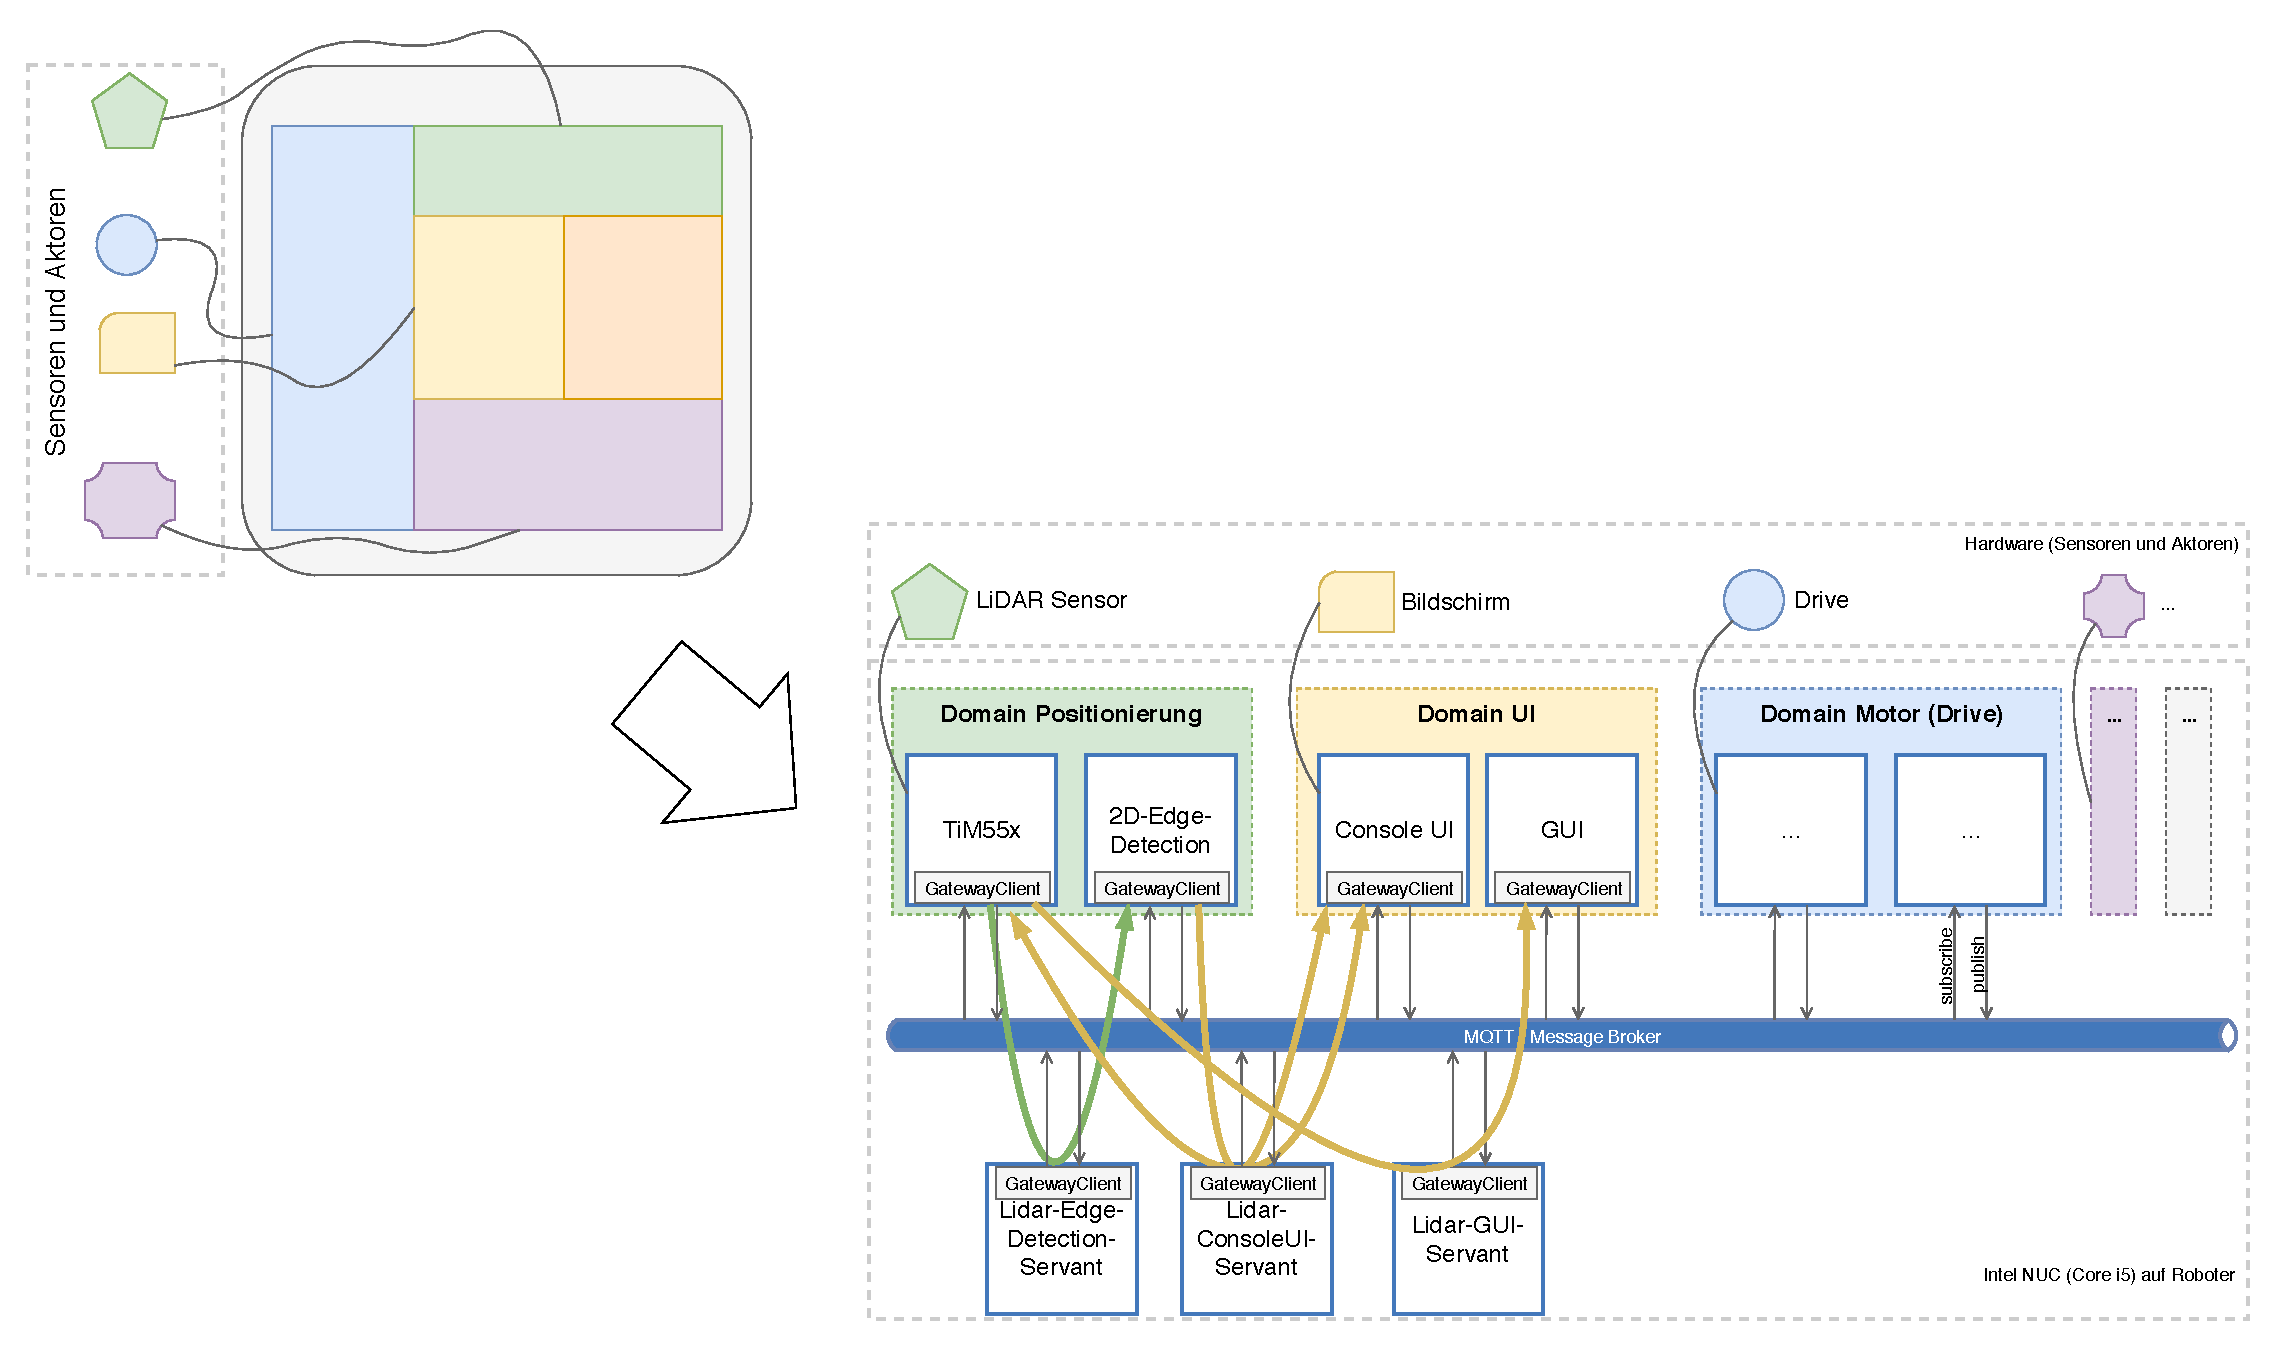
\includegraphics[width=0.95\textwidth]{img/titelbild.pdf}			% Titelbild definieren
\end{textblock}

\begin{textblock}{154}(28,135)
	\begin{picture}(150,2)
		\put(0,0){\color{bfhgrey}\rule{150mm}{2mm}}
	\end{picture}
\end{textblock}
\color{black}

% Institution / Titel / Untertitel / Autoren / Experten:
%---------------------------------------------------------------------------
\begin{flushleft}

\vspace*{115mm}

\fontsize{26pt}{28pt}\selectfont 
\titel	\\						% Titel aus der Datei vorspann/titel.tex lesen
\vspace{2mm}

\fontsize{16pt}{20pt}\selectfont\vspace{0.3em}
\untertitel 			\\				% Untertitel eingeben
\vspace{5mm}

\fontsize{10pt}{12pt}\selectfont
\textbf{\ArtDerArbeit} \\		% eingeben
\vspace{3mm}

% Abstract (eingeben):
%---------------------------------------------------------------------------
%\begin{textblock}{150}(28,190)
%\fontsize{10pt}{12pt}\selectfont
%[Kurztext (Abstract) einfügen, falls gewünscht] \\ 
%Dieses Dokument dient als Vorlage für die Erstellung von Berichten nach den Richtlinien der BFH. Die Vorlage ist in \LaTeX{} %erstellt und unterstützt das automatische Erstellen von diversen Verzeichnissen, Literaturangaben, Indexierung und Glossaren. %Dieser kleine Text ist eine Zusammenfassung über das vorliegenden Dokument mit einer Länge von 4 bis max. 8 Zeilen. \\
%Das Titelbild kann in den Zeilen 157/158 der Datei template.tex ein- oder ausgeschaltet werden.
%\end{textblock}

\begin{textblock}{150}(28,225)
\fontsize{10pt}{17pt}\selectfont
\begin{tabbing}
	xxxxxxxxxxxxxxx\=xxxxxxxxxxxxxxxxxxxxxxxxxxxxxxxxxxxxxxxxxxxxxxx \kill
	Studiengang:	\> \studiengang		\\
	Autor:		\> \autor		\\
	Betreuer:	\> \betreuer		\\
	Auftraggeber:	\> \auftraggeber	\\
	Experten:	\> \experte		\\
	Datum:		\> \today		\\
\end{tabbing}

\end{textblock}
\end{flushleft}

\begin{textblock}{150}(28,280)
\noindent 
\color{bfhgrey}\fontsize{9pt}{10pt}\selectfont
Berner Fachhochschule | Haute école spécialisée bernoise | Bern University of Applied Sciences
\color{black}\selectfont
\end{textblock}


\end{titlepage}		% activate for Titelseite mit Bild
%\include{vorspann/versionen}
%\cleardoubleemptypage
%\setcounter{page}{1}
%\cleardoublepage
%\phantomsection 
\addcontentsline{toc}{chapter}{Management Summary}
\chapter*{Management Summary}
Die Höhere Fachschule für Technik Mittelland (HFTM) nimmt seit einigen Jahren mit dem Team ,,Solidus'' am internationalen RoboCup in der ,,Logistics League'' mit Erfolg teil. In der ,,Logistics League'' geht es darum, mit selber entwickelten Roboter in einer Produktionsanlage (Smart Factory) die Zwischenschritte - also die Logistik - zu automatisieren. Der Roboter bekommt beispielsweise den Auftrag aus dem Lager zur Anlage 1 Material zu bringen, oder von Anlage 2 die produzierten Teile abzuholen und ins Lager oder zu einer weiteren Produktionsanlage zu bringen. Die Roboter-Software ist mittlerweile relativ ausgereift für den aktuellen Cup. Das Team besteht jedes Jahr aus neuen Studenten die keinen vertieften Hintergrund in der Softwareentwicklung haben. Sie übernehmen die bestehende Code-Base vom vorherigen Team und müssen diese an die neuen Gegebenheiten anpassen und erweitern. Die historisch gewachsene, monolithische Architektur der Software wirkt diesen Anforderungen aber entgegen.

Das Ziel ist es, eine Softwarearchitektur und ein Entwicklungsvorgehen zu entwerfen, welche die Anforderungen an kurze Einarbeitungszeit und Flexibilität erfüllt. Fordert die geringere Effizienz der Umsetzung zwar mehr Ressourcen auf der Zielplattform, steigert sie dafür aber die Effizienz bei der Entwicklung.

In einer zeitgemässen Tool-Chain für die Entwicklung und einer Architektur basierend auf Microservices wurde die Anbindung eines Sensors (LiDAR) realisiert. Die einzelnen Schritte wurden so dokumentiert, dass sie in Schulungsunterlagen Verwendung finden können. So kann sichergestellt werden, dass zukünftige Entwicklungen voneinander abgekapselt in eigenständigen Microservices stattfinden können und somit keine direkte Abhängigkeit untereinander aufweisen. Die Kopplung und Datenkonversion der einzelnen Services wird mit Hilfe von domänenspezifischen Verbindern (Servants) realisiert.

Die exemplarische Entwicklung aus der Umsetzung zeigt, wie man künftig an der HFTM die Optimierung und Weiterentwicklung der Software angehen könnte. Das resultierende Dokument zu dieser Arbeit wurde so erfasst, dass es den zukünftigen HFTM-Studenten als Leitfaden dienen kann. Die Ausgangslage und die Umsetzung erlauben einen fliessenden Übergang in die neue Architektur.
%\cleardoubleemptypage
%---------------------------------------------------------------------------

% Table of contents
%---------------------------------------------------------------------------
\tableofcontents
%\cleardoublepage
%---------------------------------------------------------------------------

% Main part:
%---------------------------------------------------------------------------
\chapter{Einleitung}
\pagenumbering{arabic}
Die Studenten der Höheren Fachschule für Technik Mittelland (\acrshort{hftm}) aus der Studienrichtung Systemtechnik nehmen seit einigen Jahren am internationalen RoboCup teil. Dazu kommt ein Roboter mit selbst entwickelter Hard- und Software zum Einsatz. Unter dem Team-Namen ,,Solidus'' spielen die Studenten am RoboCup bereits an der Spitze mit (2. und 3. Platz). Das Team besteht nebst dem Dozenten Alain Rohr jedes Jahr aus neuen Studenten die keinen vertieften Hintergrund in der Softwareentwicklung haben. Sie übernehmen die bestehende Code-Base vom vorherigen Team und müssen diese an die neuen Gegebenheiten anpassen und erweitern. Beispielsweise ändert sich jährlich die Umgebung (Lichtverhältnisse, etc.), die Cup-Regeln und es müssen neue Sensoren oder Aktoren integriert werden. Die historisch gewachsene, monolithische Architektur der Software wirkt diesen Anforderungen aber entgegen.
Sie baten die BFH um Hilfe beim Software-Engineering. Es geht in dieser Arbeit also darum, ein Design für die Roboter-Software zu entwerfen, so dass die Studenten unabhängig voneinander entwickeln können.
\section{RoboCup}
Der RoboCup ist ein Wettbewerb, der seit 1997 jährlich ausgetragen wird \cite{wikipedia-robocup}. Ursprünglich ging es hauptsächlich darum, Roboter zu entwickeln, die gegeneinander Fussball spielen. Das langfristige Ziel dieses Wettbewerbs \cite{wikipedia-roboterfussball}: 
\begin{formal}
im Jahr 2050 den menschlichen Weltmeister in einem gewöhnlichen Fussballspiel zu schlagen
\end{formal}
Es kommen jedoch immer neue Ligen dazu. Der aktuelle Stand an Ligen für den RoboCup 2018 ist in Screenshot aus Abbildung \ref{fig:robocup_ligen} ersichtlich.
\begin{figure}[H]
	\centering
	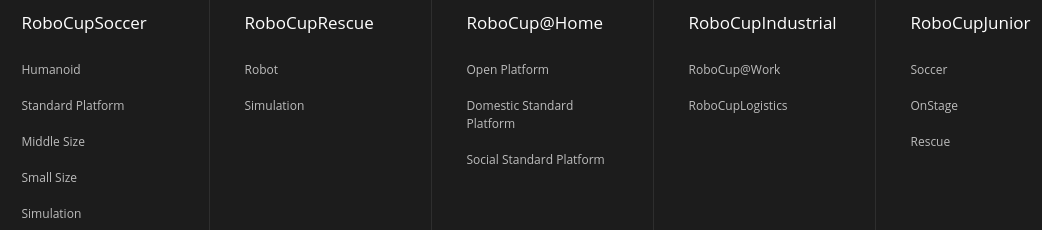
\includegraphics[width=\textwidth]{img/robocup-ligen.png}
	\caption{RoboCup Ligen, Screenshot von \cite{www.robocup.org}}
	\label{fig:robocup_ligen}
\end{figure} 
So gibt es beispielsweise in der Disziplin ,,RoboCupSoccer'' die Liga ,,Humanoid''. Die Roboter aus dieser Liga sind auch in den Medien hierzulande sehr bekannt. Im Bild \ref{fig:robocup_fussball} ist ein solcher Humanoid beim Fussballspielen am RoboCup zu sehen.
\begin{figure}[H]
	\centering
	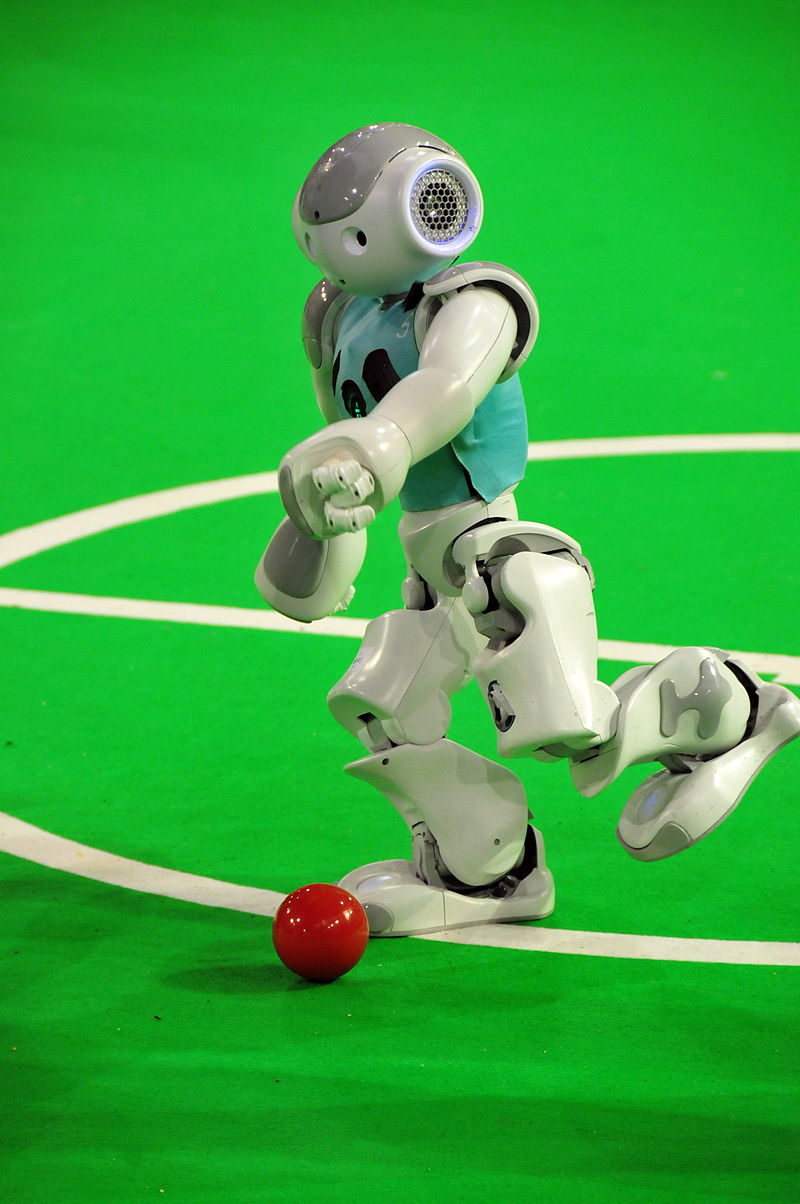
\includegraphics[width=0.2\textwidth]{img/robocup-humanoid.jpg}
	\caption{Roboter beim Fussball spielen. Quelle: Ralf Roletschek / roletschek.at \cite{robocup2013}}
	\label{fig:robocup_fussball}
\end{figure}
\subsection{RoboCupLogistics}
Seit 2012 gibt es am RoboCup die Liga ,,Logistics'', die wie folgt spezifiziert ist \cite{wikipedia-robocup}:
\begin{formal}
	Ziel dieser Liga ist die Entwicklung von autonom agierender Roboter zur Steuerung des Material- und Informationsflusses in industriellen Produktionsanlagen.
\end{formal}
Es spielen zwei Teams gegeneinander mit jeweils 3 Robotern. Auf dem  Spielfeld (Abbildung \ref{fig:robocup_spielfeld}) sind pro Team zufällig sieben Maschinen  aufgestellt. Diese müssen von den Robotern erkundet werden. Dafür hat jede Maschine vorne und hinten einen eindeutigen 2D-Code aufgedruckt, dem so genannten AR Tag (Prinzip ähnlich einem QR-Code). Jede Maschine repräsentiert eine Station in einer Produktionsanlage (einer ,,smart factory''). An jeder Station können Gegenstände zugebracht und auf der gegenüberliegenden Seite entnommen werden. Kontrolliert, überwacht und bewertet wird das Spiel von der ,,Referee Box''. Von ihr werden die 'Active orders' (Bestellungen) verwaltet und publiziert, die die Roboter auf dem Spielfeld umsetzen müssen. Sie koordiniert auch die Maschinen auf dem Spielfeld, zu denen die Roboter fahren müssen, um Gegenstände zu bringen und abzuholen.
\begin{figure}[H]
	\centering
	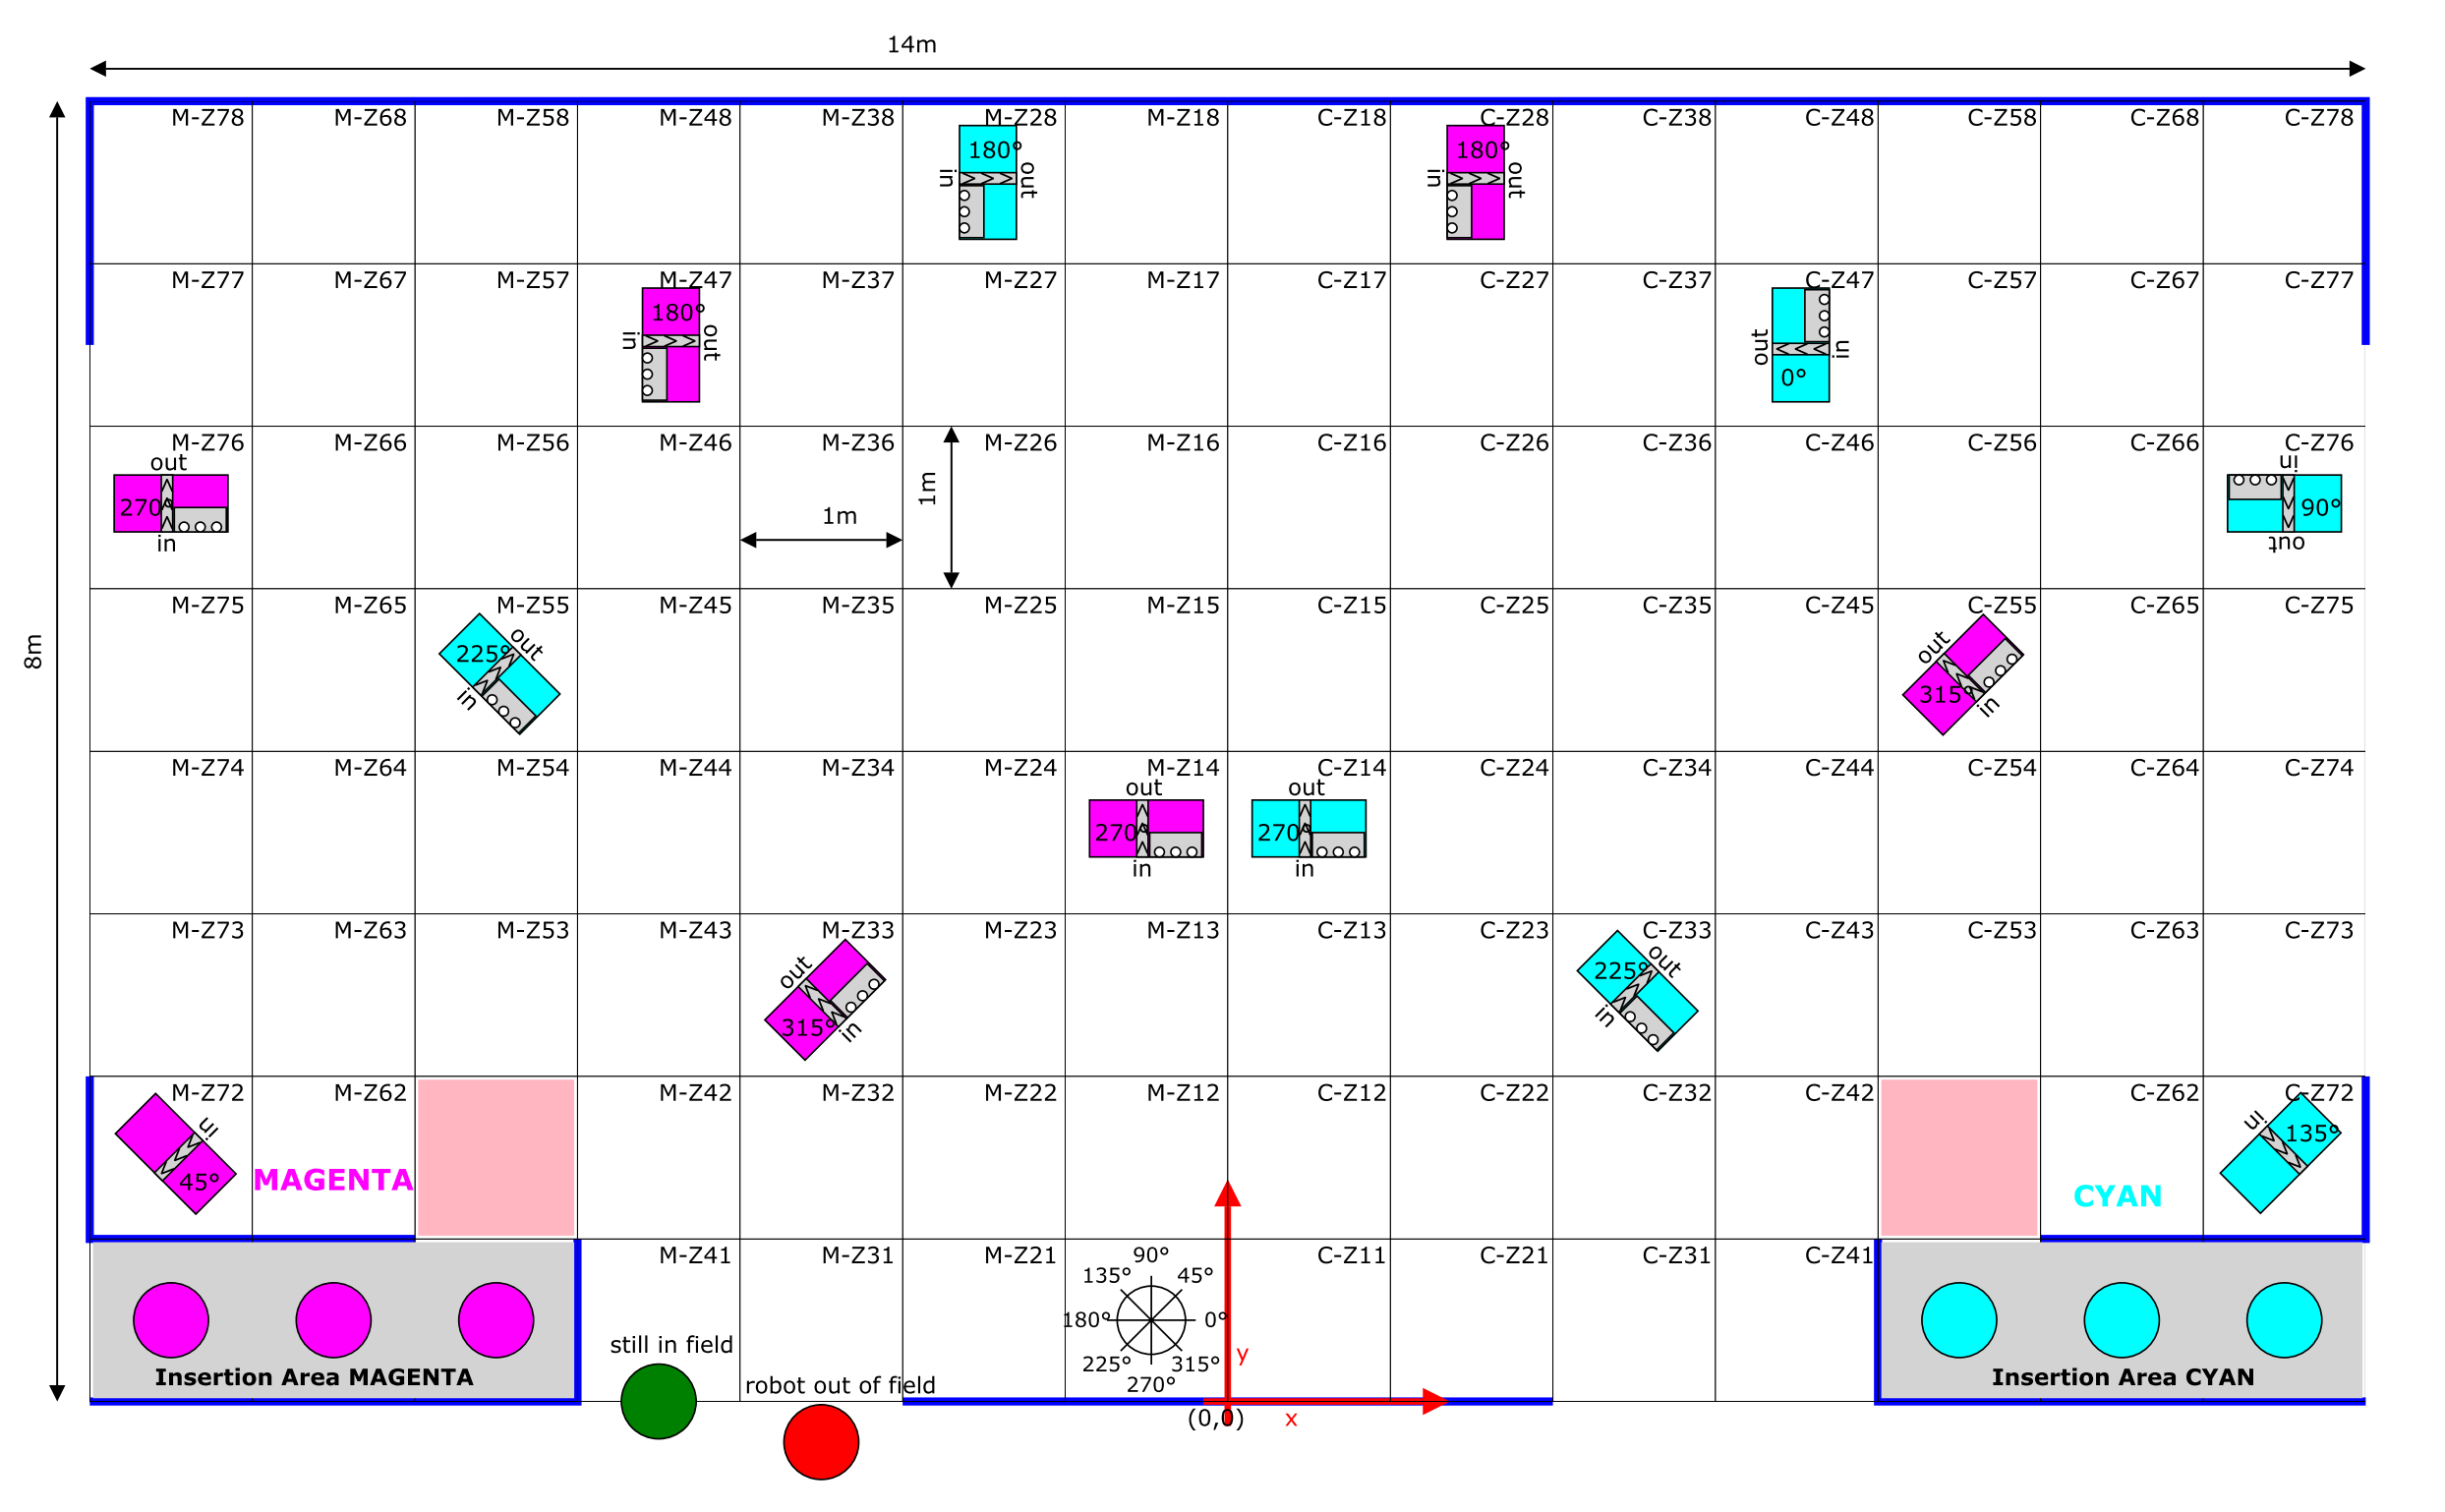
\includegraphics[width=0.75\textwidth]{img/robocup-spielfeld-2d.png}
	\caption{Spielfeld mit möglicher Aufstellung der Maschinen: Quelle: robotics-erlangen.de \cite{robotics-erlangen.de}}
	\label{fig:robocup_spielfeld}
\end{figure}

Die verwendeten Roboter in dieser Liga basieren auf der ,,Robotino''-Plattform  von Festo (Abbildung \ref{fig:robotino}), die den Wettbewerb auch mit den Maschinen und anderem sponsern. Auf dieser Roboterplattform können verschiedene Sensoren, Aktoren und Computer-Systeme angebaut werden.
\begin{figure}[H]
	\centering
	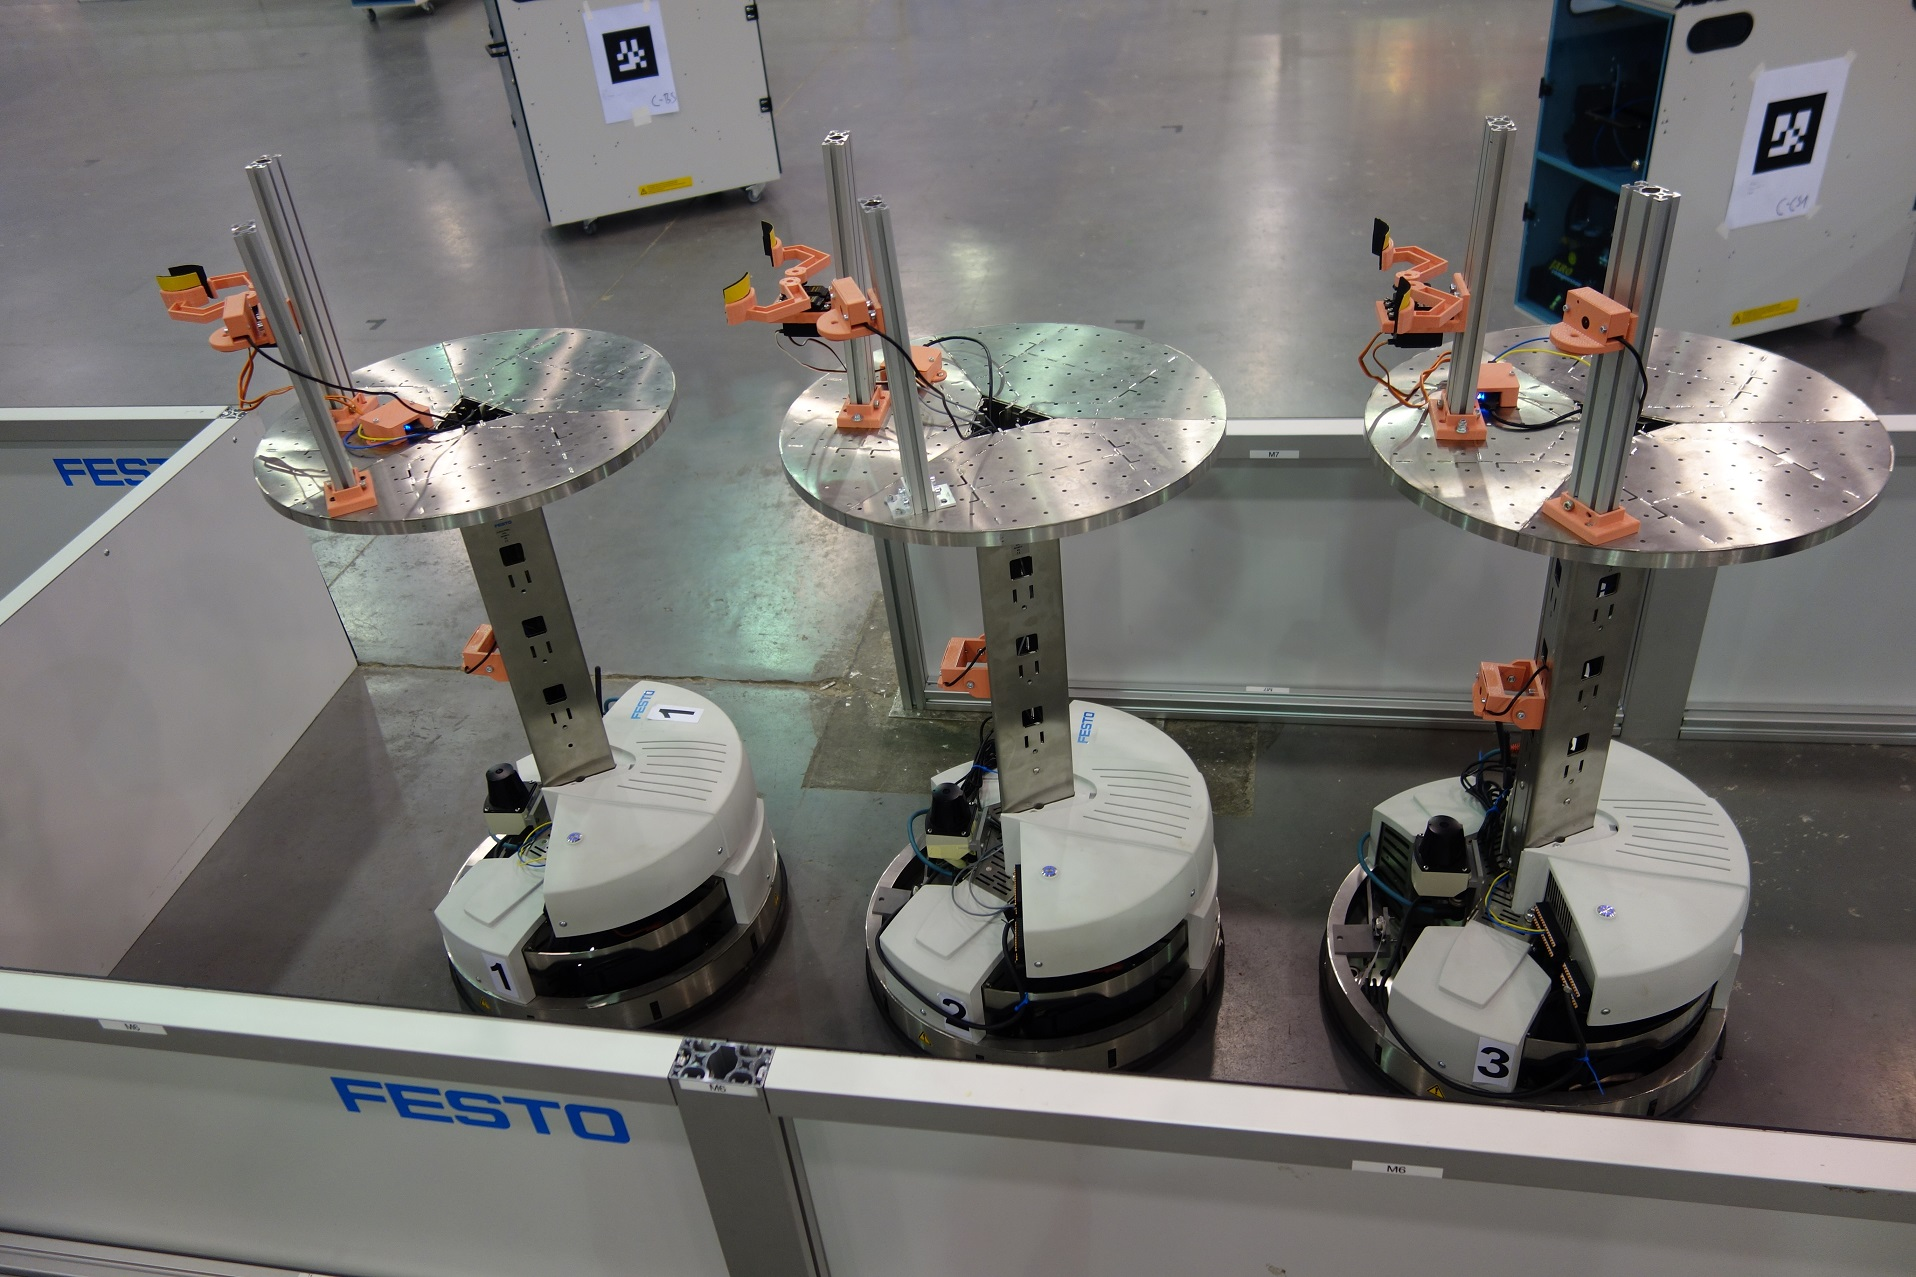
\includegraphics[width=0.5\textwidth]{img/robotino_v3.jpg}
	\caption{Robotino v3 für die Logistics League\cite{robotino}}
	\label{fig:robotino}
\end{figure}



\section{\acrshort{lidar}}
Diese Arbeit zeigt anhand eines \acrshort{lidar}-Sensors, wie ein mögliches Software-Design für den Roboter aussehen kann. Doch was ist \acrshort{lidar}?
\begin{formal}
	Lidar ist eine dem Radar verwandte Methode zur optischen Abstands- und Geschwindigkeitsmessung sowie zur Fernmessung atmosphärischer Parameter. Statt der Radiowellen wie beim Radar werden Laserstrahlen verwendet. \cite{wikipedia-lidar}
\end{formal}
Meistens versteht man unter em Begriff \acrshort{lidar} gleich einen Sensor, wie er auch in dieser Arbeit verwendet wird. Sie messen nicht nur in eine Richtung, sondern fast die ganze Umgebung um den Sensor herum. Der in dieser Arbeit verwendete TiM55x kann 270° der Umgebung ausmessen. Solche Sensoren kommen beispielsweise bei Fahrzeugen mit Autopilot (Bsp. Tesla) zum Einsatz um die Hindernisse in der Umgebung zu erkennen. Im Prinzip funktionieren solche Sensoren ähnlich wie eine Radar-Bodenstation in der Luftfahrt: Über ein drehendes Element (bei \acrshort{lidar} einen Spiegel) werden kontinuierlich Laserstrahl-Impulse ausgesendet. Wenn sich ein Objekt in der Nähe des Sensors befindet, trifft dieser Laserstrahl das Objekt und ein Teil davon wird reflektiert. Die Reflexion detektiert der Sensor und errechnet daraus die resultierende Distanz zum Objekt.
\begin{figure}[H]
	\centering
	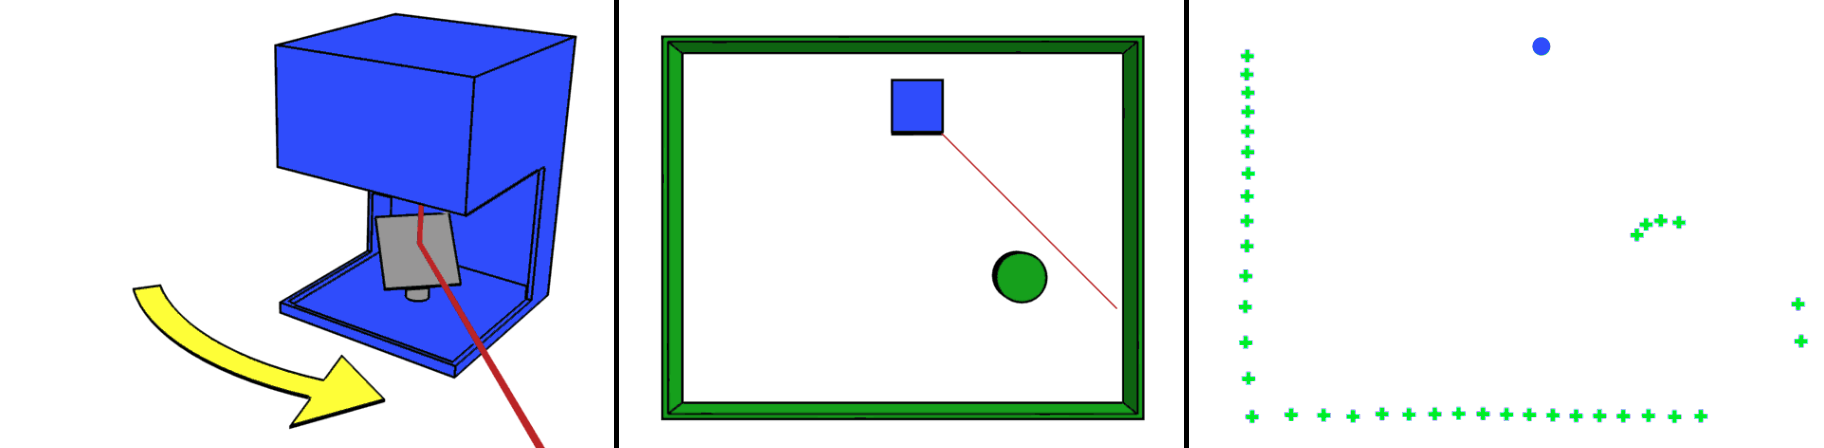
\includegraphics[width=0.7\textwidth]{img/lidar-principle.png}
	\caption{Prinzip 2D-Abtastung mit Lidar \cite{wikipedia-lidar}}
	\label{fig:lidar-principle}
\end{figure}


\subsection{SICK TiM55x}
\label{chap:tim55x}
Die Funktionsweise des verwendeten Sensors ist im Datenblatt vom Hersteller SICK wie folgt beschrieben \cite{tim55x-techinfo}:
\begin{formal}
Der TiM5xx sendet mit einer Laserdiode gepulste Laserstrahlen aus. Trifft ein solcher Laserpuls auf ein Objekt oder eine Person, wird er an dessen Oberfläche reflektiert. Die Reflexion wird im Empfänger des TiM5xx von einer Fotodiode registriert. Der TiM5xx nutzt die SICK-eigene HDDM-Technologie (High Definition Distance Measurement). Bei diesem Messverfahren wird ein Messwert durch die Mittelwertbildung mehrerer Einzelpulse gebildet. Aus der Laufzeit, die das Licht von der Aussendung des Strahls bis zum Empfang der Reflexion benötigt, berechnet der TiM5xx die Entfernung zum Objekt. Dieses Prinzip der ,,Pulslaufzeitmessung'' wird in ähnlicher Form von Radarsystemen benutzt.

Mit einem rotierenden Spiegel lenkt der TiM5xx die ausgesendeten Laserstrahlen ab und tastet damit die Umgebung radial ab. Die Messungen werden intern von einem Winkelkodierer in regelmässigen Winkelschritten ausgelöst. Eine komplette Rotation stellt einen Messvorgang (Scan) dar. Der TiM5xx arbeitet mit einer Scanfrequenz von 15 Hz, d. h. er durchläuft 15 Messvorgänge pro Sekunde und stellt die Messergebnisse fortlaufend in Echtzeit über die Ethernet-Schnittstelle zur Verfügung.
\end{formal}

Wir erhalten also von diesem Sensor 15 Mal Sekunde eine komplette Messung mit 270 Distanzen und der dazugehörigen Genauigkeit. Diese Messwerte sind wie im Datenblatt beschrieben wie folgt zu verstehen: Der erste Messwert erhalten wir bei -45° und der letzte bei 225° (siehe dazu Abbildung \ref{fig:lidar}). Der TiM55x-Sensor ist an der Robotino-Plattform so verbaut, dass 90° vorne entspricht. Weshalb der Hersteller negative Werte im Koordinatensystem verwendet hinterfragen wir nicht weiter. Die zu entwickelnde Software soll also genau diesen Winkel-Bereich zur Verfügung stellen - so steht er auch im Datenblatt.
\begin{figure}[H]
	\centering
	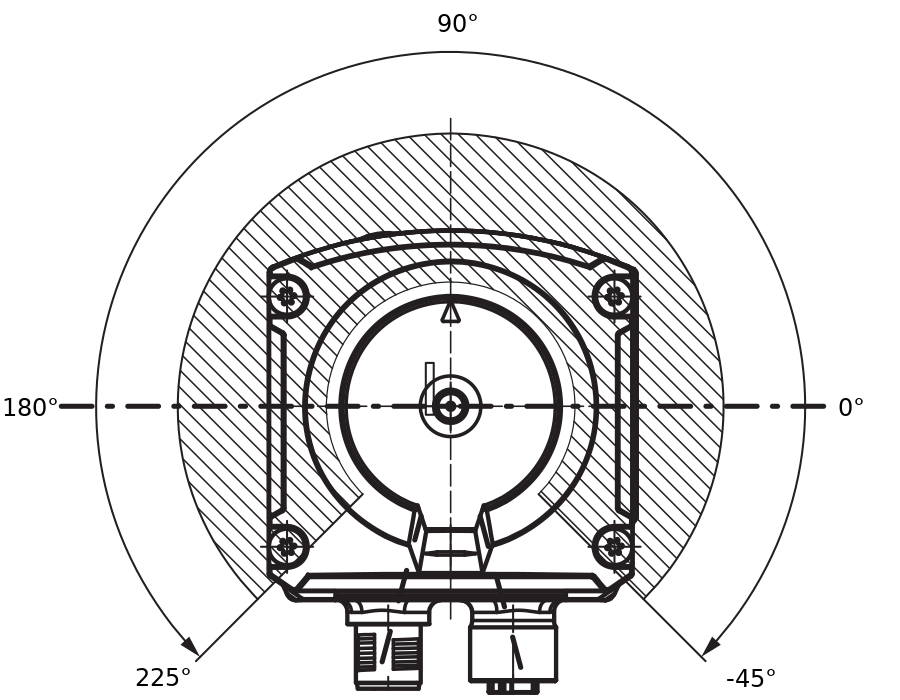
\includegraphics[width=0.5\textwidth]{img/lidar-coordinate.png}
	\caption{\acrshort{lidar}: Draufsicht / Koordinatensystem}
	\label{fig:lidar}
\end{figure}

%\pagenumbering{arabic}
\chapter{Ziel}
\label{chap:software-design}
In diesem Kapitel wird ein mögliches Design für den RoboCup erläutert.
\section{Einführung}
In den nachfolgenden Abschnitten soll gezeigt werden, wie man die einzelnen Systeme des Roboters in Services (Positionierung, Drive-Einheit, Greifsystem, etc.) unterteilt und dazwischen simple Schnittstellen realisieren kann.
Jede einzelne Komponente im System verwendet zum Austausch mit Anderen den Systemweiten Message Broker.

\section{Monolith vs. Microservice}
Man hört es heute an jedem Entwickler-Event, liest es in verschiedenen Zeitschriften, egal ob für Entwickler oder System-Administratoren: der Weg zum Ziel sollen Microservices sein, sie sollen Monolithen ablösen. Viele kleine Services statt einen grossen, verzahnten und schwierig wartbaren Moloch.
In \cite{informatik-aktuell-microservices} findet sich ein passendes Statement zur monolithischen Applikation:
\begin{formal}
	Selbstverständlich startet keine Neuentwicklung als ,,grosser Monolith". Anfangs ist die Anwendung schlank, leicht zu erweitern und gut zu verstehen – die Architektur adressiert die Probleme, die das Team zu dieser Zeit hat. Im Laufe der Monate entsteht mehr und mehr Code. Es werden Schichten definiert, Abstraktionen gefunden, Module, Services und Frameworks eingeführt, um die wachsende Komplexität in den Griff zu bekommen.
	
	Bereits bei mittelgrossen Anwendungen (etwa eine Java-Anwendung mit mehr als 50.000 LOC\footnote{Lines of Code}) werden monolithische Architekturen langsam unangenehm. Das gilt vor allem für Anwendungen, die hohe Anforderungen an die Skalierbarkeit stellen. Aus der schlanken Neuentwicklung entwickelt sich das nächste Legacy-System, über das folgende Generationen von Entwicklern fluchen werden.
\end{formal}
\subsection{Vorteile von Microservices}
Die Vorteile von Microservices sprechen für sich. Deshalb setzen auch die Internetriesen wie Netflix, Amazon, eBay und Uber seit einiger Zeit darauf. Hier ein Auszug der wichtigsten Punke aus der selben Quelle\cite{informatik-aktuell-microservices}, die für den Roboter interessant sind:
\begin{formal}
	\begin{itemize}
		\item
		Aufgrund ihrer geringen Grösse benötigt man wenig Boiler-Plate Code und keine schwergewichtigen Frameworks.
		\item
		Sie lassen sich unabhängig voneinander deployen. Continuous Delivery bzw. Deployment lässt sich damit sehr viel einfacher realisieren.
		\item
		Die Architektur unterstützt die Arbeit in mehreren, unabhängigen Teams.
		\item
		Es ist pro Service möglich, die jeweils „beste“ Programmiersprache zu wählen. Man kann ohne grosses Risiko auch mal eine neue Sprache, ein neues Framework oder ähnliches ausprobieren. Man sollte es dabei nur nicht übertreiben.
		\item
		Da sie klein sind, lassen sie sich auch jederzeit mit vertretbarem Aufwand durch eine Neuentwicklung ablösen.
		\item
		Microservices kommen der agilen Entwicklung entgegen. Ein neues Feature, von dessen Erfolg beim Kunden man noch nicht überzeugt ist, lässt sich nicht nur schnell entwickeln – es lässt sich auch schnell wieder wegwerfen.
	\end{itemize}
\end{formal}

Folgendes Argument kommt noch dazu: Durch die Tatsache, dass die Schnittstellen klar definiert sind, lassen sich an einem Service jederzeit einfache Blackbox-Tests durchführen: Man versorgt den Service an der Schnittstelle mit den Testdaten und prüft, ob die richtigen Daten raus kommen. Diesen Punkt werden wir später in diesem Dokument anhand des Lidar-Services anschauen.
\subsection{Nachteile von Microservices}
Natürlich gibt es mit Microservices auch Nachteile, die man nicht verschweigen sollte:
\begin{itemize}
	\item
	Durch die Kapselung in einzelne Komponenten (und sogar eigene Java VMs) braucht es  grundsätzlich mehr Ressourcen. Vor allem in Bezug auf Memory und Netzwerkverkehr.
	\item
	Objekte werden in einer YAML-/JSON-/(XML)-Struktur serialisiert übers Netzwerk versendet. Der Consumer-Service muss diese dann wieder in Objekte ,,abfüllen'' (marshalling/unmarshalling). Dieses Serialisieren und Deserialisieren ist ziemlich ,,teuer'' was die CPU Performance anbelangt.
	
\end{itemize}


\section{Architektur}
\label{sec:Architektur}
Das historisch gewachsene, monolithische Design (Schaubild \ref{fig:architecture_current_highlevel}) soll also umgebaut werden.
\begin{figure}[H]
	\centering
	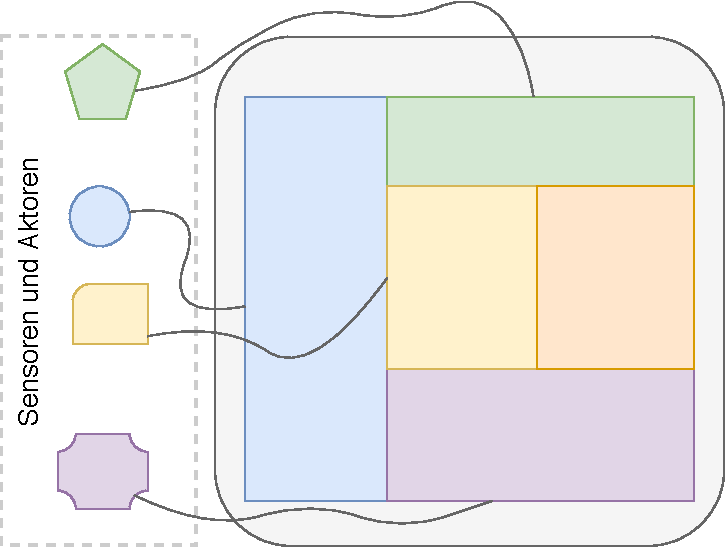
\includegraphics[width=0.3\textwidth]{img/architecture-highlevel-today.pdf}
	\caption{Bestehende Architektur (plakatives Schaubild)}
	\label{fig:architecture_current_highlevel}
\end{figure}
Beim bestehenden Design kommunizieren einige Komponenten bereits heute über das \acrshort{mqtt}-Protokoll (Details zu \acrshort{mqtt} im Abschnitt \ref{sec:mqtt}). In der neuen Architektur soll dies komplett in den Mittelpunkt rücken und für den Datenaustausch der einzelnen Services zuständig sein. Es gäbe auch andere Event-/Message-Busse, die dafür verwendet werden könnten (Bsp. \Gls{ros}). In Diskussionen mit dem Betreuer und dem Auftraggeber hat sich aber herausgestellt, dass \Gls{ros} zu viele Herausforderungen mit sich bringt. Das RoboCup-Team aus Deutschland beisse sich daran auch die Zähne aus. \\
\acrshort{mqtt} ist durch die Verwendung in Heimautomationen bereits weit verbreitet und es gibt Libraries für unterschiedliche Programmiersprachen und eine grosse Community dafür. Vor allem aber kennen die Studenten der HFTM dieses Protokoll bereits. \\ Es sollen also Microservices entstehen, die nur genau eine Aufgabe erfüllen. Einige werden nur das hardware-spezifische Protokoll (hier \acrshort{lidar}) in die \acrshort{mqtt}-Welt adaptieren. Andere werden Berechnungen mit den Daten ausführen und die Resultate wieder bereitstellen. \Glspl{service} kennen sich untereinander nicht, sie wissen nichts von der Existenz anderer \glspl{service}. Damit die einzelnen \Glspl{service} miteinander kommunizieren können, kommen Verbinder zum Einsatz,  so genannte \Glspl{servant}. Diese kennen die Schnittstellen (\gls{contract} bzw. \acrshort{api}) der zu bedienenden Services. Wir werden dieses Konzept in den nachfolgenden Kapitel am Beispiel des \acrshort{lidar} anschauen.

\begin{figure}[H]
	\centering
	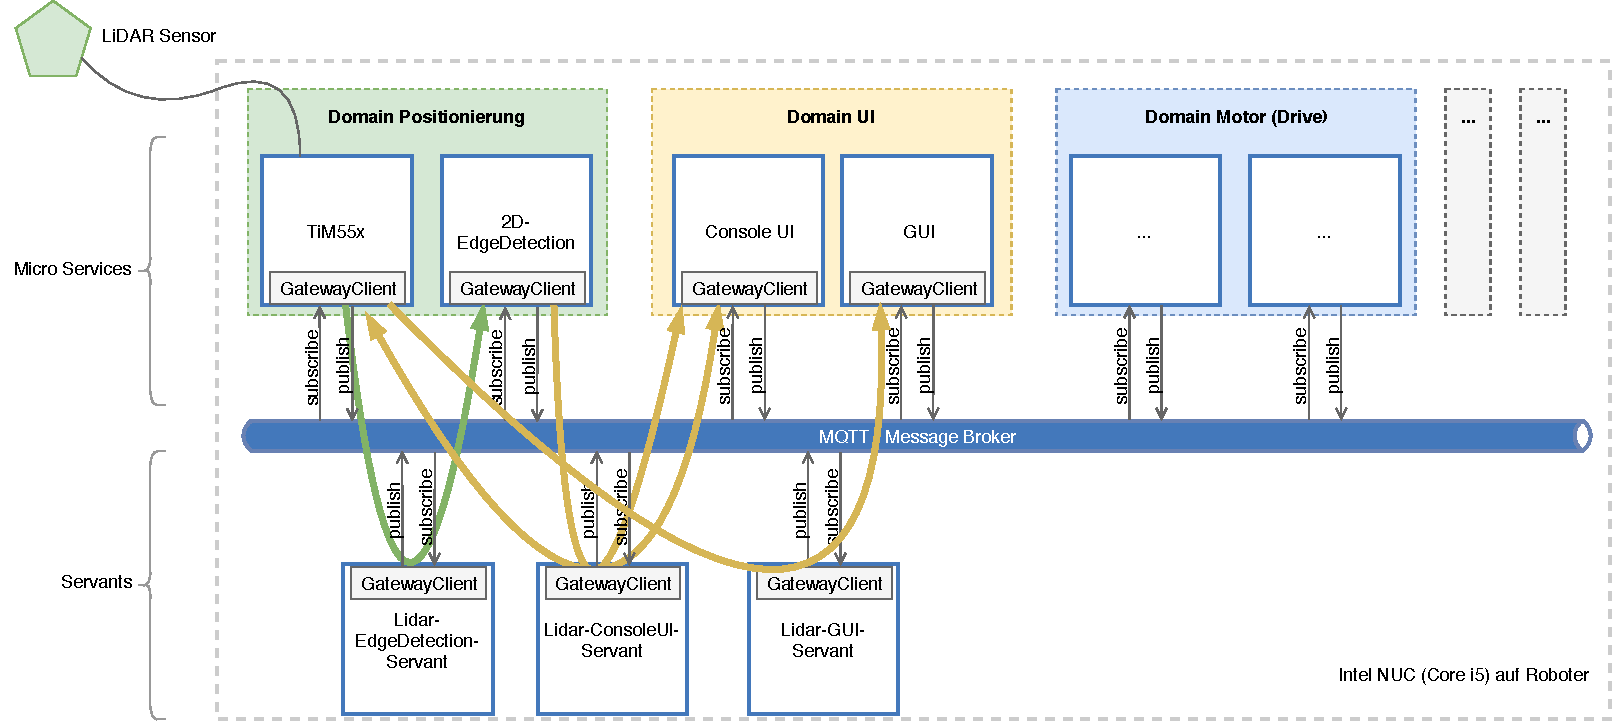
\includegraphics[width=\textwidth]{img/architecture-highlevel.pdf}
	\caption{Architektur in Domains}
	\label{fig:architecture_highlevel}
\end{figure}

Die Abbildung \ref{fig:architecture_highlevel} zeigt wie die einzelnen Services durch die Servants verbunden werden. Ein Servant kann mehrere Services ,,verbinden'' dafür gibt es keine Regel. Es gibt beispielsweise einen \Gls{servant}, der die gelieferten Daten vom TiM55x-Service konvertiert und dem EdgeDetection-Service gibt. Fürs UI könnten aber sowohl Daten vom TiM55x-Service als auch vom EdgeDetection-Service relevant sein. Dazu wird der Lidar-UI-Servant die Daten entsprechend zusammenführen und dem UI-Service übergeben. Der UI-Service dient hier nur als Beispiel. In der Praxis - also im Kontext des RoboCups - werden diese Informationen vielleicht an einem Service mit Fahrlogik übergeben.

\subsection{Ausführung der Services, Hardware-Ressourcen}
Die Idee ist grundsätzlich, dass jeder Service für sich ausgeführt wird. Im Kontext der nach diesem Leitfaden entwickelten Services bedeutet das aber, dass für jeden Service eine eigene Java VM gestartet wird. Je nach Anzahl der Services wird auf der Zielplattform, dem Intel NUC, aber zu wenig Arbeitsspeicher für dieses Vorhaben zur Verfügung stehen. Deshalb ist vorgesehen, dass es pro Domäne einen 'Domänen-Runner' gibt, der alle Services einer Domäne in einer JVM startet.

\section{Aufbau eines Services, Begriffe}
\label{sec:isePattern}
Jeder Service im System soll sich an in diesem Abschnitt beschriebenen Grundsatz halten. Als Student der BFH mit Mobile Computing als Schwerpunkt lernt man bei Reto Koenig folgendes Muster für die MQTT-Topics kennen: Intent, Status und Event. Was das bedeutet wird in den nächsten Abschnitten beschrieben. Die \acrshort{mqtt}-Topics stellen das \acrshort{api} für den jeweiligen Service dar. \\ Die nachfolgenden Teilabschnitte basieren auf dem englischen README aus dem Github-Projekt von Reto Koenig \cite{ch.quantasy.mqtt.gateway}.

\subsection{Payload}
In der Payload der Topics - also der Nachricht - befindet sich nicht nur ein Wert wie bisher, sondern eine Struktur (JSON, YAML, XML, etc.). Wir verwenden hier \acrshort{yaml}, damit man die Daten mit einem handelsüblichen MQTT-Client (z.B. MQTTlens\cite{mqtt-lens} oder MQTTfx\cite{mqttfx}) für den Mensch sehr einfach verständlich anzeigen kann (siehe Listing \ref{lst:examplePayload}). Denn \acrshort{yaml} ist frei von eckigen, spitzigen und runden Klammern, Tags und Kommas. Jede Payload enthält mindestens einen Zeitstempel mit der Systemzeit als die Meldung ins MQTT-System eingespiesen wurde. Der Zeitstempel einer Nachricht von einem Service wird bei Bedarf vom Servant ausgewertet und je nach Anwendungsfall weiterverarbeitet.

\begin{lstlisting}[caption={Beispiel einer MQTT-Payload}, label={lst:examplePayload}]
---
- timeStamp: 65630678285913
  command: "SINGLE_MEASUREMENT"
\end{lstlisting}

\subsection{Unit}
Als \gls{unit} wir eine Instanz eines Services bezeichnet. Beispielsweise wird der TiM55x-Service für jeden vorhandenen \acrshort{lidar}-Sensor als eine individuelle Instanz gestartet. Das sind also unterschiedliche Units. Jede Instanz bzw. Unit hat sein eigenes MQTT Basis-Topic.

\subsection{Intent}
Kann ein Service Befehle über die \acrshort{mqtt}-\acrshort{api} entgegennehmen, so werden diese über das Topic '\gls{intent}' dem Service mitgeteilt. Dafür muss sich der Service auf dieses Topic abonnieren ('subscribe'). Pro Service gibt es nur ein Intent-Topic. \\ Es hat sich herausgestellt, dass ein Design mit mehreren Intent-Topics pro Services unpraktikabel ist. Beispielsweise sind sie plötzlich abhängig untereinander, dh. es muss zuerst das eine Intent und später das andere gesendet werden. Das ist fast nicht handhabbar wenn verschiedene Teilnehmer mit einem Service interagieren. Ein ähnliches Konzept verfolgt auch Google bei Android. Zuerst wird der komplette Intent definiert (also die Absicht was das System tun soll und wie) und dann wird er versendet.

\subsection{Status}
Mehrheitlich statische Informationen stellt ein Service unter dem Basis-Topic '\gls{status}' zur Verfügung. Am Beispiel des \acrshort{lidar}-Sensors gehören hier jegliche Informationen über den Sensor in diese Kategorie rein: Firmwarestand, Konfiguration, State des Sensors (Sensor wird initialisiert / Messung läuft / Standby / etc.). Unter diesem Topic kann eine beliebige Baumstruktur aufgebaut werden.

\subsection{Event}
Alle Informationen, die eventgesteuert sind oder auftreten können, klassifizieren wir in diese Kategorie. Die Messwerte des Sensors gehören beispielsweise in dieses Topic.

\subsection{Description}
Im Topic '\gls{description}' beschreibt ein Service bzw. eine \acrshort{unit} beim Aufstarten das angebotene \acrshort{api}. Das ermöglicht für Entwickler die Anbindung an andere Komponenten. Die Description des APIs ist vor allem für die Entwicklung von Services relevant, die nicht den im nachfolgenden Kapitel beschriebenen \ctexttt{GatewayClient} verwenden.

\subsection{Beispiele}
Ein Topic in unserem sieht also Beispielsweise wie folgt aus:

\begin{minipage}{\linewidth}
\begin{verbatim}
Robocup/Lidar/U/192.168.91.2@kicm-fedora.localdomain/S/connection
         ^    ^       ^                              ^  ^
         |    |       |                              |  |
         |    |       |                              |  '--- Topic unterhalb 'Status'
         |    |       |                              '------ Status Trennzeichen
         |    |       '------------------------------------- Name der Unit / Instanz
         |    '--------------------------------------------- Unit Trennzeichen
         '-------------------------------------------------- Name des Services
\end{verbatim}
\end{minipage}

\subsubsection{Beispiel mehrere \acrshort{lidar}-Sensoren}
Wenn wir mehrere Sensoren verwenden, arbeiten die Instanzen des TiM55x-Services beispielsweise in diesen Basis-Topics:
\begin{itemize}
	\item \texttt{Robocup/Lidar/U/192.168.91.11@mainpc.robot1.hftm.localdomain/...}
	\item \texttt{Robocup/Lidar/U/192.168.91.22@mainpc.robot1.hftm.localdomain/...}
	\item \texttt{Robocup/Lidar/U/192.168.91.33@mainpc.robot1.hftm.localdomain/...}
\end{itemize}

\subsubsection{Beispiel \acrshort{lidar}-Sensoren auf einem Roboter verteilt auf mehrere Computer}
Wenn wir mehrere Sensoren verwenden, arbeiten die Instanzen des TiM55x-Services beispielsweise in diesen Basis-Topics:
\begin{itemize}
	\item \texttt{Robocup/Lidar/U/192.168.91.11@mainpc.robot1.hftm.localdomain/...}
	\item \texttt{Robocup/Lidar/U/192.168.91.22@secondpc.robot1.hftm.localdomain/...}
	\item \texttt{Robocup/Lidar/U/192.168.91.33@secondpc.robot1.hftm.localdomain/...}
\end{itemize}
\chapter{Grundlagen}
\label{chap:voraussetzungen}
Dieses Kapitel soll oberflächlich einige Dinge erklären, die für diese Arbeit vorausgesetzt werden.
\section{Apache Maven}
\label{chap:maven}
Maven ist ein Tool um den Build-Prozess von Software zu unterstützen. Es bietet beispielsweise Unterstützung fürs Managen der Abhängigkeiten, fürs Testing und zur Paketierung. Die zu entwickelnden Services aus Kapitel \ref{chap:beispielimplementation} verwenden Maven vor allem für das Dependency-Management. Konkret ist Maven in diesem Projekt für folgendes zuständig:
\begin{itemize}
	\item
	Libraries müssen nicht manuell heruntergeladen und ins Projekt aufgenommen werden.
	\item
	Versionen der Libraries sind zentral definiert. Ein Upgrade einer Library auf eine neue Version lässt sich somit an einem Ort erledigen.
	\item
	Paketierung der Services/Applikationen als Jar-Datei.
\end{itemize}
Um Maven zu verwendet erstellt man in der verwendeten Entwicklungsumgebung (\acrshort{ide}) ein 'Maven-Projekt'. Zentral in einem Maven-Projekt ist die Datei \texttt{pom.xml} (\acrshort{pom} steht für \acrlong{pom}). Sie definiert wie oben erläutert die Umgebung für das Java-Projekt.

\subsection{Dependencies}
Maven verwendet so genannte Repositores um Libraries anzuziehen. Repositories können lokal oder remote sein. Dependencies/Libraries sucht man beispielsweise auf \texttt{mvnrepository.com}. Alle Libaries in diesem Repository kennt Maven automatisch und kann diese herunterladen. Heruntergeladen werden die Libraries (als Jar paketiert) in das lokale Repository, also in den Ordner \texttt{.m2} im Home-Verzeichnis des ausführenden Benutzers. In dieser Arbeit ist das also \path{/home/mkilchhofer/.m2/repository} (Fedora Linux) und unter Windows wird das in \path{C:\Users\mkilchhofer\.m2\repository} sein.

Als kurzes Beispiel hier eine Demonstration zur Einbindung von Log4j2.
\begin{enumerate}
	\item Auf mvnrepository nach ,,Log4j Core'' suchen.
	\item Version auswählen (hier zum Beispiel ,,2.11.0'')
	\item XML-Struktur (Abbildung \ref{fig:mvnrepository-example}) im \texttt{pom.xml} in den Sub-Baum \texttt{<dependencies>} einfügen (Listing \ref{lst:maven-example-simple})
\end{enumerate}

\begin{figure}[H]
	\centering
	\includegraphics[width=0.7\textwidth]{img/voraussetzung/mvnrepository-example.png}
	\caption{Code zum kopieren von \texttt{mvnrepository.com}}
	\label{fig:mvnrepository-example}
\end{figure}

\begin{lstlisting}[language=XML, caption={Simples Beispiel wie ein pom.xml aussieht},label={lst:maven-example-simple}]
<?xml version="1.0" encoding="UTF-8"?>
<project /* ... (generiert die IDE) ... */>
	<modelVersion>4.0.0</modelVersion>
	<artifactId>lidar-hardware-service</artifactId>
	<groupId>info.kilchhofer.bfh</groupId>
	<version>1.1-SNAPSHOT</version>
	<packaging>jar</packaging>

	<dependencies>
		<dependency>
			<groupId>org.apache.logging.log4j</groupId>
			<artifactId>log4j-core</artifactId>
			<version>2.11.0</version>
		</dependency>
	</dependencies>
</project>
\end{lstlisting}
Maven übernimmt dann über die \acrshort{ide} den Rest und lädt das Jar und nötigenfalls die Sources an die erforderlichen Orte herunter.
\subsection{Maven Lifecycle}
In jeder aktuellen \acrshort{ide} ist Maven sehr gut eingebunden. So taucht bei einem maven-managed Projekt in der \acrshort{ide} \textit{\Gls{intellij}} folgende Komponente an der rechten Seite auf:
\begin{figure}[H]
	\centering
	\includegraphics[scale=0.5]{img/voraussetzung/maven-lifecycle-ide2.png}
	\caption{Maven Lifecycle in der \acrshort{ide}}
	\label{fig:maven-ide}
\end{figure}
Durch das Auswählen der jeweiligen Lifecycle-Phase mit anschliessendem Drücken auf den Play-Knopf wird der entsprechende Task ausgeführt. Was die einzelnen Phasen (Tasks) genau machen ist folgender Tabelle \ref{tab:mavenLifecycle} zu entnehmen.

\begin{table}[H]
	\centering
	\begin{tabular}{lp{13cm}} \toprule
		\textbf{Lifecycle} & \textbf{Beschreibung}\\ \midrule
		\texttt{clean}     & Alle generierten Objekte (namentlich 'Artefakte') und das Verzeichnis '\path{target}' werden gelöscht.\\ \midrule
		\texttt{validate}  & Validieren ob alle Projekt-Infos vorhanden und korrekt sind (vor allem pom.xml prüfen).\\ \midrule
		\texttt{compile}   & Kompiliert den Source-Code des Projekts. Syntax-Fehler im Verzeichnis '\path{src/main/..}' lassen diese Phase Fehlschlagen. Die Tests aus dem Verzeichnis '\path{src/test/..}' werden in dieser Phase noch nicht berücksichtigt. Syntax-Fehler in den Unit-Tests beeinflussen das erfolgreiche Abschliessen dieser Phase nicht.\\ \midrule
		\texttt{test}	   & Führt die Tests gegen den kompilierten Source-Code aus. Diese Tasks endet erfolgreich, wenn die Syntax aller Tests fehlerfrei sind und die Tests erfolgreich durchgeführt werden können.\\ \midrule
		\texttt{package}   & Paketiert den generierten Byte-Code in ein verteilbares Archiv (Bsp. Jar)\\ \midrule
		\texttt{verify}	   & Prüft die paketierten Datein mittels Integrations-Tests.\\ \midrule
		\texttt{install}   & Kopiert die paketierten Dateien in das lokale Maven Repository (\path(.m2)-Ordner), um diese als Abhängigkeit in anderen lokalen Projekten zu benutzen.\\ \midrule
		\texttt{site}      & Generiert eine Projekt-Website \\ \midrule
		\texttt{deploy}	   & Kopiert das generierte Artefakt in ein remote Maven Repository (gleich wie \texttt{install}, nur eben Remote.)				\\ \bottomrule
	\end{tabular}
	\caption{Basic Lifecycle-Phasen in Maven. Quelle: \href{https://maven.apache.org}{maven.apache.org} \cite{maven-build-lifecycle} }
	\label{tab:mavenLifecycle}
\end{table}



\section{Tests / Unit Tests}
Der zu entwickelnde Programmcode soll wie folgt automatisch auf zwei Stufen getestet werden:
\begin{itemize}
	\item Unit Tests (Klassen und Methoden)
	\item Integrationstests der verschiedenen Microservices
\end{itemize}
Die umgesetzten Tests verwenden JUnit als Framework.  Der Aufbau von JUnit Tests zeigt dieses kleine Beispiel:
\begin{lstlisting}[caption={Simples Beispiel wie JUnit funktioniert},label={lst:junit-example-simple}]
package info.kilchhofer.bfh.lidar.hardwareservice;

import org.junit.jupiter.api.Test;
import static org.junit.jupiter.api.Assertions.assertEquals;
import static org.junit.jupiter.api.Assertions.assertNotEquals;

public class SimpleTest {
	@Test
	@DisplayName("myInt durch 2 teilbar aber nicht durch 3")
	public void mySimpleTest(){
		int myInt = 1024;
		assertEquals(0, (myInt % 2));
		assertNotEquals(0, (myInt % 3));
	}
	
	@Test
	@DisplayName("Log2")
	public void mySimpleTest2(){
		int temp = (int) (Math.log(myInt) / Math.log(2));
		assertEquals(9, temp);
	}
}
\end{lstlisting}
Führt man diesen Test in der \acrshort{ide} \textit{\Gls{intellij}} aus, bekommt man folgenden Output:
\begin{figure}[H]
	\centering
	\includegraphics[width=0.7\textwidth]{img/voraussetzung/junit-example.png}
	\caption{JUnit Beispieldurchlauf}
	\label{fig:junit-example}
\end{figure}
Wie zu erwarten, schlägt der zweite Test fehl, weil der Logarithmus zur Basis 2 von 1024 natürlich 10 ist. Der Erwartungswert im Test ,,Log2'' ist aber 9.

Beispiele die sich auf den entwickelten Code beziehen gibt es im Abschnitt mit der Beispielimplementation (Kapitel \ref{chap:beispielimplementation}).

\section{Git}
Als \acrshort{vcs} setzen wir Git ein. Ins Git gehört jeglicher entwickelte Code, nicht aber Artefakte (gebuildeter Code) und IDE spezifische Einstellungen. Die entsprechenden Verzeichnisse müssen wir also in \path{.gitignore}-Datei aufnehmen.

\section{MQTT}
\label{sec:mqtt}
TODO - Stichworte: \acrshort{mqtt}, Broker, Client, publish, subscribe

\chapter{Implementation der Services am Beispiel \acrshort{lidar}}
Hier gehe ich darauf ein, wie sich das Konzept aus Kapitel \ref{chap:software-design} in Programmcode umsetzen lässt. Dabei versuche ich den Code so einfach wie möglich zu halten, da die Schüler der HFTM parallel erst an Java ausgebildet werden (siehe Anforderungen aus Abschnitt \ref{chap:aufgabenstellung}). Auf Lambda-Ausdrücke wird beispielsweise verzichtet.
\label{chap:beispielimplementation}
\section{Die Library 'GatewayClient'}
Mit der  Java-Library \ctexttt{ch.quantasy.mqtt.gateway} von Reto Koenig \cite{ch.quantasy.mqtt.gateway} lässt sich einfach ein Microservice entwickeln, der sich bereits an das Muster aus Kapitel \ref{sec:isePattern} hält (Event, Intent, Status). Man kann damit keine Messages ins MQTT publizieren die das Muster verletzen.
\begin{figure}[H]
	\centering
	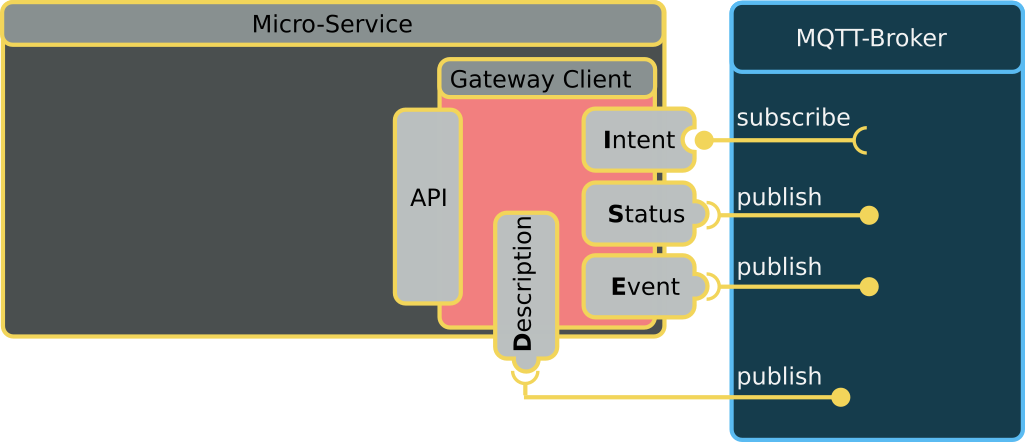
\includegraphics[width=0.6\textwidth]{img/gatewayclient.png}
	\caption{GatewayClient, ch.quantasy.mqtt.gateway\cite{ch.quantasy.mqtt.gateway}}
	\label{fig:gatewayclient}
\end{figure}
In Abbildung \ref{fig:gatewayclient} ist ersichtlich wie die Library die Basis-Topics bzw. \acrshort{api}s in Richtung MQTT-Broker zur Verfügung stellt. Die Idee hinter dem \verb|GatewayClient| ist folgende:
\begin{itemize}
	\item
	Standardisieren der Schnittstelle. Man wird zwar ,,eingeengt'' aber dafür ist die Schnittstelle einheitlich.
	\item
	Serialisierung und übertragen der Java-Objekte auf MQTT in \acrshort{yaml}-Struktur (bei den published Topics)
	\item
	Deserialisierung der YAML-Daten in die ursprünglichen Java-Objekte (bei den subscribed Topics)
	\item
	Bei jedem Verbinden zum MQTT-Broker publiziert der GatewayClient automatisch die ,,\acrshort{api}-Dokumentation''. So ist sofort ersichtlich was für eine Schnittstelle implementiert werden muss um einen weiteren \Gls{servant} an diese Schnittstelle anzuschliessen.
\end{itemize}
\subsection{Service Logik}
An den GatewayClient wird die eigentliche Service Logik angebunden. Im Github-README unterscheidet Reto Koenig\cite{ch.quantasy.mqtt.gateway} dabei wie in Abbildung \ref{fig:microService} ersichtlich zwischen 'Service Logic' und 'Service Source':
\begin{figure}[H]
	\centering
	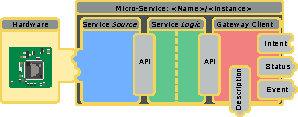
\includegraphics[width=0.6\textwidth]{img/gatewayclient-microservice.pdf}
	\caption{Micro-Service mit GatewayClient \cite{ch.quantasy.mqtt.gateway}}
	\label{fig:microService}
\end{figure}
Was das bedeutet, erklären die nächsten zwei Abschnitte.
\subsubsection{Service Source}
Unter 'Service Source' versteht man die Libraries zu einer bestimmten Hardware. Der Hersteller Tinkerforge\cite{tinkerforge-gmbh} stellt beispielsweise den Java-Code und die Library für die Anbindung ihrer Produkte bereit. Diese Kategorie beinhaltet also die Ansteuerung der Hardware aus Java. Ab diesem Punkt haben wir also Objekte und Klassen, die wir mit der 'Service Logic' ansteuern können.
\subsubsection{Service Logic}
Unter 'Service Logic' versteht man die Logik um beispielsweise einen Sensor, der bereits mittels 'Service Source' von Java aus ansprechbar ist, an den GatewayClient anzubinden.


\section{TiM55x-Service}
Der TiM55x-Service enthält (dh. \verb|import|) zum einen den GatewayClient sowie die Library der HFTM zur Dekodierung und Ansteuerung des \acrshort{lidar}s (also der 'Service Source'). Wir müssen uns folglich also um die 'Service Logic' aus Abbildung \ref{fig:lidarservice} kümmern.
\begin{figure}[H]
	\centering
	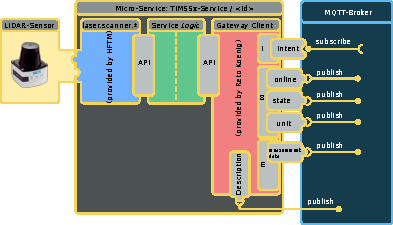
\includegraphics[width=0.6\textwidth]{img/tim55xservice.pdf}
	\caption{TiM55x-Service, Quelle des Diagramm-Templates: \cite{ch.quantasy.mqtt.gateway}}
	\label{fig:lidarservice}
\end{figure}

Der TiM55x-Service ist wie in Abbildung \ref{fig:structure_lidarservice} strukturiert. Die Idee ist, dass der Servant alles aus dem Java-Package 'binding' von unserem Service kennt, solange er auch den GatewayClient verwendet. Darin enthalten ist also die Definition der Schnittstelle und (Objekt-)Strukturen der Daten, die auf dem Event-Bus vorhanden sind.
\begin{figure}[H]
	\centering
	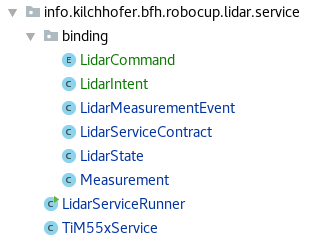
\includegraphics[scale=0.5]{img/tim55x-java-packagestructure.png}
	\caption{TiM55x-Service, Struktur}
	\label{fig:structure_lidarservice}
\end{figure}

Beginnen wir nun mit der Implementation. Der Programmcode in den nachfolgenden Abschnitten ist meist nicht vollständig, damit es übersichtlicher bleibt (mit \ctexttt{// ...} gekennzeichnet). Der vollständige Code dieser Arbeit befindet sich auf Github\cite{github-thesis}. \\
\subsection{Contracts definieren}
Als erstes wird der \Gls{contract} - also die MQTT-Topics und die Struktur der \Gls{payload} - definiert. Dazu wird die abstrakte Basis-Klasse \ctexttt{AyamlServiceContract} wie in Listing \ref{lst:lidarservice-contracts} ersichtlich erweitert.
\begin{lstlisting}[caption={TiM55x-Service - Contracts},label={lst:lidarservice-contracts}]
public class LidarServiceContract extends AyamlServiceContract {
    public final String STATE, MEASUREMENT, STATUS_STATE, EVENT_MEASUREMENT;
    // ...

    public LidarServiceContract(String instanceID) {
        super(ROBOCUP_ROOT_CONTEXT, "Lidar", instanceID);
        STATE = "state";
        MEASUREMENT = "measurement";
        STATUS_STATE = STATUS + "/" + STATE;
        EVENT_MEASUREMENT = EVENT + "/" + MEASUREMENT;
    }

    @Override
    public void setMessageTopics(Map<String, Class<? extends Message>> messageTopicMap) {
        messageTopicMap.put(INTENT, LidarIntent.class);
        messageTopicMap.put(EVENT_MEASUREMENT, LidarMeasurementEvent.class);
        messageTopicMap.put(STATUS_STATE, LidarState.class);
    }
}
\end{lstlisting}
Der TiM55x-Service verwendet also über diesen \Gls{contract} die folgenden \acrshort{mqtt}-\Glspl{topic}:
\begin{itemize}
	\item \texttt{<rootContext>/<baseClass>/U/<instanceID>/I}
	\item \texttt{<rootContext>/<baseClass>/U/<instanceID>/S/state}
	\item \texttt{<rootContext>/<baseClass>/U/<instanceID>/E/measurement}
\end{itemize}
und durch Vererbung:
\begin{itemize}
	\item \texttt{<rootContext>/<baseClass>/U/<instanceID>/S/connection}
\end{itemize}
, wobei über den Aufruf \ctexttt{super(rootContext: "Robocup", baseClass: "Lidar", instanceID)} die variablen Teile der \Glspl{topic} entsprechend gesetzt werden.

\subsubsection{Events: Messdaten}
Schauen wir uns als Beispiel noch das 'measurement'-\Gls{topic} an. Eine Momentaufnahme des \acrshort{lidar}-Sensors, also einer Messung, beinhaltet 270 Messpunkte mit dieser Struktur:
\begin{lstlisting}[caption={TiM55x-Service - Struktur der Messpunkte},label={lst:tim55x-measurement}]
public class Measurement extends AValidator {
    @Range(from = -45, to = 225)
    public int angle;
    
    @Range(from = 0, to = 10000)
    public int distance;
    
    @Range(from = 0, to = 10000)
    public int rssi;

    public Measurement(int angle, int distance, int rssi){
        this.angle = angle;
        this.distance = distance;
        this.rssi = rssi;
    }
    // ...
}
\end{lstlisting}
Über die Annotations geben wir den Variablen die möglichen Werte vor. Damit werden zum einen beim Aufstarten die \Gls{description}-Topics korrekt abgefüllt und zum anderen lassen sich die Empfangenen Werte mit dem \Gls{gatewayclient} validieren (optional). So kann man beispielsweise bestimmen, ob nicht valide Werte weiterverarbeitet werden oder nicht.
Die obigen Messpunkte einer Messung werden in einer Liste als 'LidarMeasurementEvent' übermittelt:
\begin{lstlisting}[caption={TiM55x-Service - Struktur des 'LidarMeasurementEvent'},label={lst:tim55x-measurementEvent}]
public class LidarMeasurementEvent extends AnEvent{
    @ArraySize(min = 1, max = 270)
    private ArrayList<Measurement> measurements;
    
    public LidarMeasurementEvent(ArrayList<Measurement> measurements) {
        this.measurements = measurements;
    }
    // ...
}
\end{lstlisting}

\subsubsection{Intent}
Als Intent bietet der TiM55x-Service an eine Einzel-Messung auszuführen, eine kontinuierliche Messung zu starten und diese zu stoppen. Diese drei Aktionen bietet die Library der HFTM zur Zeit an.
\begin{lstlisting}[caption={TiM55x-Service - Struktur des 'LidarIntent'},label={lst:tim55x-intent}]
import ch.quantasy.mqtt.gateway.client.message.AnIntent;
import ch.quantasy.mqtt.gateway.client.message.annotations.Nullable;

public class LidarIntent extends AnIntent {
    @Nullable
    public LidarCommand command;
    
    //..
}
\end{lstlisting}
LidarCommand ist dabei lediglich ein Enum:
\begin{lstlisting}[caption={TiM55x-Service - Struktur des 'LidarCommand'},label={lst:tim55x-lidarCommand}]
public enum LidarCommand {
    START_CONTINUOUS_MEASUREMENT, STOP_CONTINUOUS_MEASUREMENT, SINGLE_MEASUREMENT
}
\end{lstlisting}

\subsubsection{Status: Laser- / \acrshort{lidar}-State}
Im Status-Topic bietet der TiM55x-Service zusätzlich zum vererbten ConnectionStatus noch den Laser-State an. Das Problem ist hier, dass im Contract die Klasse \ctexttt{IScanOperator.State} verwendet wird, die aus einer Dependency kommt (Service Source). Die Servants im System sollten diese hardwarespezifische Klasse eigentlich nicht kennen und sollten auch nicht abhängig davon sein. So sind sie aber leider davon abhängig und benötigen diese Library über die Paketierung als \ctexttt{jar-with-dependencies}. Dies wird im Kapitel \ref{sec:separatebindings} weiter diskutiert.
\begin{lstlisting}[caption={TiM55x-Service - Struktur des 'LidarState'},label={lst:tim55x-lidarState}]
//..
import laser.scanner.IScanOperator;

public class LidarState extends AStatus{
    public IScanOperator.State state;

    public LidarState(IScanOperator.State state) {
        this.state = state;
    }

    public LidarState() {
    }
}
\end{lstlisting}

\subsubsection{Übersicht über den fertigen Contract}
Der Programmcode von oben führt uns zu dieser Struktur für den TiM55x-ServiceContract (Abbildung \ref{fig:tim55x-binding-overview}). Das Muster (Event, Intent Status) ist hier gleich ersichtlich.
\begin{figure}[H]
	\centering
	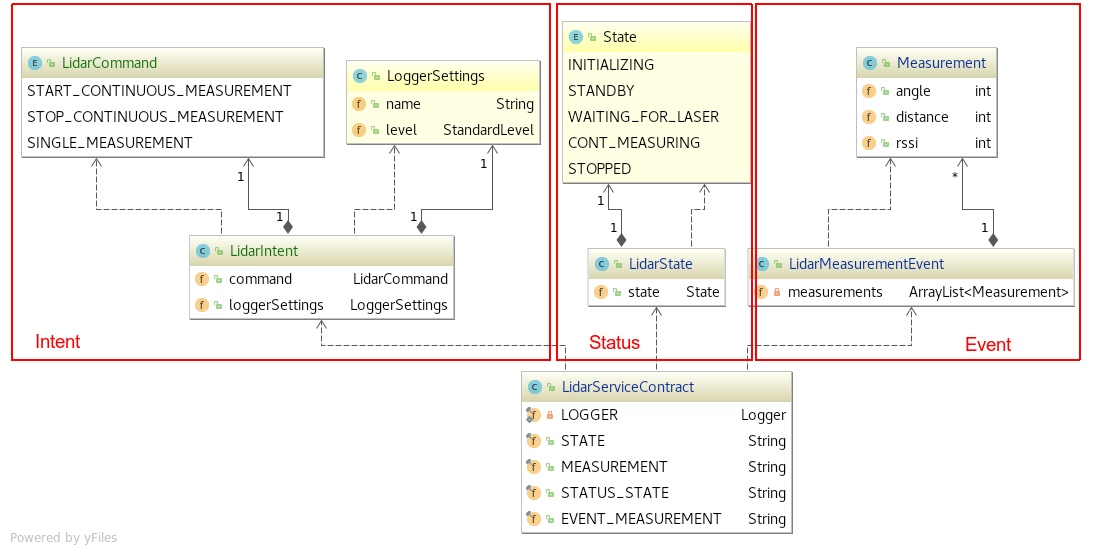
\includegraphics[width=0.7\textwidth]{img/tim55x-binding-overview.png}
	\caption{Übersicht über das Zusammenspiel des Contracts im Package binding}
	\label{fig:tim55x-binding-overview}
\end{figure}

\subsection{Service Logik implementieren}
\label{sec:service-logik-tim55x}
Die nachfolgenden Code-Snippets aus Listing \ref{lst:TiM55x-service} zeigen den Aufbau des TiM55x-Service. Der GatewayClient wird über \ctexttt{<LidarServiceContract>} mit dem \Gls{contract} instantiiert, damit er die Schnittstelle kennt. Bei den Zeilen mit \ctexttt{IScanListener ... }, \ctexttt{IScanOperator ...} sowie \ctexttt{new TiM55x(...)} sieht man die Anbindung an die Sensor-Libary. Andersherum bei \ctexttt{MessageReceiver} und \ctexttt{gatewayClient.subscribe} die Anbindung mit dem GatewayClient an \acrshort{mqtt}. Der Code zeigt also schön, wie die 'Service Logic' beide ,,Welten'' zusammenklebt.

\lstinputlisting[caption={Aufbau TiM55x-Service},language=Java,label={lst:TiM55x-service}]{listings/lidarservice_new.java}

Beim Verarbeiten des Intents wird es spannend. Wir können mit dem GatewayClient ein Set von Messages erhalten - sprich wir können mehrere Intents zum exakt gleichen Zeitpunkt erhalten. Wir nehmen hier einfach den letzten (also den neuesten) im Set. Wie sich ein Service diesbezüglich verhalten soll, muss je nach Situation geklärt werden. Hier wird es sicherlich keinen Sinn machen, den Laser beispielsweise zu aktivieren und gleich wieder zu deaktivieren. Oder wenn zwei Anfragen für eine Einzel-Messung kommen, reicht es auch, die letzte Anfrage auszuführen, es hören ja alle zu und bekommen die Messwerte geliefert.

\subsection{Beispiel-Message am MQTT-Broker}
Der Programmcode aus den Abschnitten oben, wird folgende Nachrichten auf dem MQTT-Broker erzeugen:
\begin{lstlisting}
Robocup/Lidar/U/127.0.0.1@kicm-fedora.localdomain/I ---
- timeStamp: 1528384864556686000
  command: "SINGLE_MEASUREMENT"

Robocup/Lidar/U/127.0.0.1@kicm-fedora.localdomain/E/measurement ---
- timeStamp: 1528384864699874545
  measurements:
- angle: -45
  distance: 278
  rssi: 154
- angle: -44
  distance: 288
  rssi: 157
  .
  . (nicht komplett)
  .
- angle: 224
  distance: 1130
  rssi: 182
\end{lstlisting}

\subsection{Tests mit JUnit}
Der TiM55x-Service verwendet als '\Gls{service-source}' die Library der HFTM. Theoretisch müsste hier also die '\Gls{service-logic}' per Unit-Test getestet werden. Ein einfacher Unittest ist aber ohne die beiden Libraries '\Gls{service-source}' und '\Gls{gatewayclient}' zu mocken fast nicht möglich und auch nicht sehr aussagekräftig. Deshalb werden am Service lediglich Service-Tests mit JUnit durchgeführt. Dies geschieht automatisch in der Maven Lifecycle-Phase \textit{integration-test}.
\subsubsection{Service-Test initialisieren}
Initialisiert wird das Setup wie folgt:
\begin{lstlisting}[caption={Service-Test Setup für den TiM55x-Service},label={lst:integrationstest-tim55x-setup}]
public class TiM55xServiceIntegrationTest {
    // ..
    static int LIDAR_PORT = 2112;
    static String LIDAR_IP = "127.0.0.1";
    static String MQTT_BROKER = "tcp://127.0.0.1:11234";
    //.. 
    @BeforeAll
    public static void setUpBeforeClass() {
        mqttURI = URI.create(MQTT_BROKER);
        //..
        try {
            // Embedded Broker
            // https://github.com/andsel/moquette/blob/master/
            // embedding_moquette/src/main/java/io/moquette/
            // testembedded/EmbeddedLauncher.java
            EmbeddedBrokerLauncher embeddedBrokerLauncher = new EmbeddedBrokerLauncher();

            // Start Hardware Mock
            Runnable r = new Runnable() {
            @Override
                public void run() {
                    try {
                        new HardwareMock(LIDAR_PORT);
                    } catch (InterruptedException e) {
                        LOGGER.error("InterruptedException: ", e);
                    }
                }
            };
            new Thread(r).start();
            Thread.sleep(2000);

            // GatewayClient
            gatewayClient = new GatewayClient<TiM55xServiceTestContract>(mqttURI, mqttClientName, new TiM55xServiceTestContract(instanceName));
            gatewayClient.connect();
            Thread.sleep(1000);
        } catch (Exception e) {
            fail("Exception during Setup");
        } 
    }
    
    // Hier folgen die Test cases
}
\end{lstlisting}
Wir starten also gleich zwei Umsysteme damit - einen Mock-Service (siehe Kapitel \ref{chap:tim-mock}) und einen MQTT-Broker (Moquette MQTT broker \cite{moquette-mqtt-broker}). Damit lässt sich das ganze auch wieder automatisieren. Wir müssen also nicht von Hand erst einen Sensor ans Netzwerk anschliessen, den Broker starten und danach erst den Test ausführen. Der JUnit-Test erledigt alles für uns. So wird sichergestellt, dass bei jedem Release aussagekräftige Tests durchgeführt werden. Bei einer Anpassung am Code, sieht man also sofort, dass etwas nicht mehr stimmt.

\subsubsection{Test-Szenario 'TiM55x-Service starten'}
Kommen wir also zum ersten Test-Szenario: den TiM55x-Service starten.
\begin{lstlisting}[caption={TiM55x Startup-Test}]
@Test
@DisplayName("Start TiM55x Service")
public void bringTiM55xServiceUp() {
    try {
        tiM55xService = new TiM55xService(mqttURI, "SomeTestingWithTiM55x", "SomeTestingWithTiM55x",LIDAR_IP, LIDAR_PORT);
        Thread.sleep(2000);
    } catch (Exception e) {
        fail("Exception during TiM55x Startup");
    }
}
\end{lstlisting}
Startet der Service ohne Exception nehmen wir an, dass er korrekt aufgestartet ist. Denn er wirft sofort Exceptions wenn die Sensor- oder \acrshort{mqtt}-Seite nicht da ist.

\subsubsection{Test-Szenario 'Status-Topic prüfen'}
Jetzt wird es spannender. Wir prüfen nun, wie sich der Status vom TiM55x-Service verhält. Dazu abonnieren wir das entsprechende Topic beim MQTT-Broker und prüfen ob der Status auf  'online' gewechselt hat (\ctexttt{assertEquals(...)}). Falls nicht, schlägt dieser Test fehl.

Das Problem ist, dass die Tests warten müssen, bis wir eine Antwort über den \acrshort{mqtt}-Broker erhalten. Es ist also nicht ein synchroner Aufruf wie beispielsweise bei einer bekannten HTTP-Anfrage (Request, Response), sondern eben asynchron (Publish, Subscribe, siehe \ref{sec:publish-subscribe}). Das heisst für uns, dass die Antwort irgendwann kommen kann und nicht direkt beim Aufruf von \ctexttt{gatewayClient.subscribe(...)}. Deshalb bauen wir einen \ctexttt{CountDownLatch} ein, den wir auf 1 stellen. Beim Empfangen (\texttt{messageReceived}) dekrementieren wir dem Counter. Die Zeile \ctexttt{latch.await(100, TimeUnit.SECONDS)} wartet bis dieser Counter auf 0 steht und blockiert ansonsten maximal für 100 Sekunden, bevor der Test ausgewertet (\texttt{assertEquals}) wird.

\begin{lstlisting}
@Test
@DisplayName("Subscription to Connection Status Topic")
public void subscribeStatus() throws InterruptedException {
    CountDownLatch latch = new CountDownLatch(1);

    MessageReceiver messageReceiver = new MessageReceiver() {
        @Override
        public void messageReceived(String topic, byte[] payload) throws Exception {
            LOGGER.trace("Payload: " + new String(payload));
            resultConnectionStatus = (ConnectionStatus) gatewayClient.toMessageSet(payload, ConnectionStatus.class).last();
            latch.countDown();
        }
    };

    this.gatewayClient.subscribe(tempLidarServiceContract.STATUS_CONNECTION, messageReceiver);
    latch.await(100, TimeUnit.SECONDS);
    assertEquals("online", resultConnectionStatus.value);
}
\end{lstlisting}

\section{ConsoleUI-Service}
\label{sec:ConsoleUI-Service}
Nachdem wir nun im Grundsatz wissen, wie ein Service aufgebaut wird, fallen die Erklärungen in diesem Abschnitt geringer aus.\\ Ein einfacher UI Service soll uns ein Command Line Interface zur Verfügung stellen. Die Struktur sieht analog vom TiM55x-Service aus:
\begin{figure}[H]
	\centering
	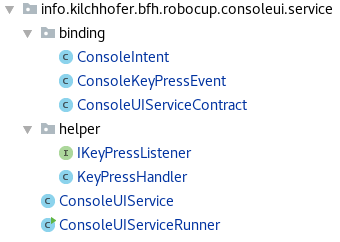
\includegraphics[scale=0.5]{img/consoleui-java-packagestructure.png}
	\caption{ConsoleUI-Service, Struktur}
	\label{fig:structure_consoleuiservice}
\end{figure}
\subsection{Contracts definieren}
\subsubsection{Event}
Der Service wird jeden Tastendruck als einzelnen Event publizieren (Listing \ref{lst:consoleui-KeyPressEvent}).
\begin{lstlisting}[caption={KeyPressEvent für den ConsoleUI-Service},label={lst:consoleui-KeyPressEvent}]
public class ConsoleKeyPressEvent extends AnEvent{
    @StringForm
    @StringSize (min=1, max=1)
    public Character character;

    public ConsoleKeyPressEvent(Character character){
        this.character = character;
    }

    public ConsoleKeyPressEvent() {
    }
}
\end{lstlisting}
\subsubsection{Intent}
Als Intent bietet der Service an, einen String ins Terminal zu schreiben (Listing \ref{lst:consoleui-intent}). Hier ist zusätzlich noch ein weiterer Intent verfügbar: loggerSettings. Damit kann man den Loglevel zur Laufzeit ändern. Er soll lediglich als Beispiel dienen, aber trotzdem eine sinnvolle Funktion anbieten. Über die Annotations wird in diesem \Gls{contract} festgelegt, dass sie nicht vorhanden sein müssen (\texttt{@Nullable}). Wir könnten also auch einen Intent an diesen Service senden, der nur einen Timestamp enthält. Diesen erzwingt der GatewayClient.
\begin{lstlisting}[caption={Intent für den ConsoleUI-Service},label={lst:consoleui-intent}]
public class ConsoleIntent extends AnIntent{
    @Nullable
    public LoggerSettings loggerSettings;

    @Nullable
    @StringForm
    public String consoleMessage;

    public ConsoleIntent(String consoleMessage){
        this.consoleMessage = consoleMessage;
    }

    public ConsoleIntent(){
    }
}
\end{lstlisting}
\subsection{Service Logik implementieren}
Die Logik ist wieder analog wie beim TiM55x-Service: wir haben einen Teil der ankommende Intents verarbeitet und einen keyPressListener, der bei jedem Tastendruck einen Event zum \acrshort{mqtt}-Broker sendet.
\begin{lstlisting}[caption={Service Logik für den ConsoleUI-Service},label={lst:consoleui-service-logic}]
//..
// Intent Handling
this.intentReceiver = new MessageReceiver() {
    @Override
    public void messageReceived(String topic, byte[] payload) throws Exception {
        for(ConsoleIntent intent : gatewayClient.toMessageSet(payload, ConsoleIntent.class)){
            if (intent.consoleMessage != null){
                System.out.println(intent.consoleMessage);
            }

            if (intent.loggerSettings != null){
                intent.loggerSettings.configure();
            }
        }
    }
};
this.gatewayClient.connect();
this.gatewayClient.subscribe(gatewayClient.getContract().INTENT + "/#", this.intentReceiver);

// Event / Console Handling
IKeyPressListener keyPressListener = new IKeyPressListener() {
    @Override
    public void keyPressed(Character character) {
        gatewayClient.readyToPublish(gatewayClient.getContract().EVENT_KEYPRESS, new ConsoleKeyPressEvent(character));
    }
};
keyPressHandler = new KeyPressHandler(keyPressListener);
Thread keyPressHandlerThread = new Thread(keyPressHandler);
keyPressHandlerThread.start();
\end{lstlisting}

\section{TiM55x-zu-ConsoleUI-Servant}
Im Abschnitt \ref{sec:Architektur} wird erläutert, dass Services untereinander keine Abhängigkeit haben. Der Servant aber hat nun Abhängigkeiten zu den bedienenden Services. So müssen wir also diese Abhängigkeiten im POM (\texttt{pom.xml}) spezifizieren, damit wir den Inhalt der entsprechenden Jars auf dem ClassPath zur Verfügung haben und die Bindings benützen können:
\begin{lstlisting}[caption={Dependencies vom TiM55x-zu-UI-Servant},label={lst:servant-dependencies},language={XML}]
<dependency>
  <groupId>info.kilchhofer.bfh</groupId>
  <artifactId>robocup-consoleui-service</artifactId>
  <version>20180607.0</version>
</dependency>
  <dependency>
  <groupId>info.kilchhofer.bfh</groupId>
  <artifactId>robocup-lidar-service</artifactId>
  <version>20180607.0</version>
  <classifier>jar-with-dependencies</classifier>
</dependency>
\end{lstlisting}
\label{sec:servant-dependencies}
Die Übersicht über den Contract vom TiM55x-Service (Abbildung \ref{fig:tim55x-binding-overview}) zeigt, wie die State-Klasse aus der 'Service Source' bis zum Contract / Binding nach vorne durchdrückt. Dies wurde bewusst so beibehalten um dies hier zu diskutieren. Aufgrund dieser Tatsache brauchen wir wie im Listing \ref{lst:servant-dependencies} auf Zeile 10 ersichtlich das Komplette Jar mit allen Dependencies (Fat Jar). Vergleich 20 kB zu 4.2 MB. Das sollten wir also in Zukunft vermeiden und beim Contract nur Objekte definieren, die wir auch im Binding-Package haben.
\begin{lstlisting}[caption={Grössenvergleich Jar zu Fat-Jar vom TiM55x-Service},label={lst:tim55x-service-fat-jar},language={none}]
$ pwd
/home/mkilchhofer/.m2/repository/info/kilchhofer/bfh/robocup-lidar-service/20180612-SNAPSHOT
$ du -h *
4.0K	maven-metadata-local.xml
4.0K	_remote.repositories
20K	robocup-lidar-service-20180612-SNAPSHOT.jar
4.2M	robocup-lidar-service-20180612-SNAPSHOT-jar-with-dependencies.jar
4.0K	robocup-lidar-service-20180612-SNAPSHOT.pom
\end{lstlisting}

\subsection{Contracts definieren überflüssig}
Anders als ein Service muss ein Servant keinen spezifischen \Gls{contract} haben. Deshalb definieren wir einen ,,leeren'' Contract (Listing \ref{lst:emptyContract}). Eigentlich könnten wir den \ctexttt{AyamlServiceContract} direkt verwenden, wenn diese Klasse nicht \ctexttt{abstract} wäre. Natürlich können wir dies auch Anonym im Servant selber umsetzen, aber wir machen es analog den Services, damit ist es Projektweit identisch ist, und wir uns sofort zurecht finden.
\begin{lstlisting}[caption={,,leerer Contract'' für den Servant},label={lst:emptyContract}]
public class ConsoleUIServantContract extends AyamlServiceContract {
    public ConsoleUIServantContract(String instanceID) {
        super(ROBOCUP_ROOT_CONTEXT, "Lidar-ConsoleUI-Servant", instanceID);
    }
    @Override
    public void setMessageTopics(Map<String, Class<? extends Message>> map) {
        // none
    }
}
\end{lstlisting}
Damit kann der Servant lediglich seinen ConnectionStatus publizieren. Natürlich ist es nicht verboten weiteres anzubieten. Wir könnten beispielsweise für eine Monitoring-Software als Status anbieten, ob sich Servant und Service gefunden haben. Oder wie viele Service-Instanzen der Servant bedient. Für uns reicht es aber vorerst aus, mit dem ,,leeren'' und somit generischen Contract zu beginnen.

\subsection{Servant Logik implementieren}
Über den Trick mit \ctexttt{\path{new ConsoleUIServiceContract("+").STATUS_CONNECTION}} (Zeile 18 und 19) lassen wir uns einen String für den Subscribe-Vorgang generieren, der aufgelöst wie folgt aussieht: \\ \ctexttt{Robocup/ConsoleUI/U/+/S/connection}. Das ist also eine Wildcard Subscription. Das heisst, anstelle vom '+'-Zeichen kann alles stehen ausser einem weiteren '/'-Trennzeichen .
Durch diese Subscription bekommen wir die ConnectionStatus-Infos aus allen Instanzen vom Console-UI-Service. Bei drei Instanzen bekämen wir also die Infos aus beispielsweise folgenden Topics:
\begin{itemize}
	\item \texttt{Robocup/ConsoleUI/U/1234@kicm-fedora.localdomain/S/connection}
	\item \texttt{Robocup/ConsoleUI/U/5678@kicm-fedora.localdomain/S/connection}
	\item \texttt{Robocup/ConsoleUI/U/9876@kicm-fedora.localdomain/S/connection}
\end{itemize}

Die Implementierung des eigentlichen Services ist wieder sehr simpel:
\lstinputlisting[caption={Aufbau TiM55x-UI-Servant},language=Java,label={lst:TiM55x-UI-Servant}]{listings/servant.java}

Der Servant hat nun einige \ctexttt{MessageReceiver} mehr als die Services. Grundsätzlich so viele, wie alle Events von den zu bedienenden Services zusammen addiert. Wir wollen ja die publizierten Events und Stati im Servant abonnieren und dem anderen Service im korrekten Format als Intent publizieren.
Schauen wir uns doch mal die einfachen Receiver an:
\subsubsection{Receiver für den Connection-Status einer ConsoleUI-Instanz}
Sobald wir auf dem Topic \ctexttt{Robocup/ConsoleUI/U/+/S/connection} Nachrichten mit \ctexttt{\path{value: "online"}} in der \Gls{payload} erhalten nehmen wir diese Unit bzw. Instanz in eine Liste auf und machen eine spezifische Subscription auf den \texttt{\path{EVENT_KEYPRESS}} dieser Instanz. Wir wollen alle UIs die zuschauen möchten mit den Daten des \acrshort{lidar}s versorgen. An dieser Subscription hängen wir als Callback den \ctexttt{keyPressReceiver} an.
\begin{lstlisting}[language=Java,caption={MessageReceiver für den Connection-Status einer ConsoleUI-Instanz im Servant},label={lst:servant-uiConnectionStatusReceiver}]
this.uiConnectionStatusReceiver = new MessageReceiver() {
    @Override
    public void messageReceived(String topic, byte[] payload) throws Exception {
        LOGGER.trace("uiConnectionStatusReceiver Payload: " + new String(payload));
        ConnectionStatus connectionStatus = gatewayClient.toMessageSet(payload, ConnectionStatus.class).last();
        ConsoleUIServiceContract uiInstanceContract = new ConsoleUIServiceContract(topic, true);

        LOGGER.info("Instance '{}' is now {}", uiInstanceContract.INSTANCE, connectionStatus.value);

        if (connectionStatus.value.equals("online")) {
            gatewayClient.readyToPublish(uiInstanceContract.INTENT, new ConsoleIntent("This is a message from the Servant, we now have a connection together.") );

            uiInstances.add(uiInstanceContract);
            gatewayClient.subscribe(uiInstanceContract.EVENT_KEYPRESS, keyPressReceiver);
        } else {
            uiInstances.remove(uiInstanceContract);
            gatewayClient.unsubscribe(uiInstanceContract.EVENT_KEYPRESS);
        }
    }
};
\end{lstlisting}

In diesem \ctexttt{keyPressReceiver} sehen wir jetzt schön wie der Servants die Eigenheiten der Services ausgleicht. Oben im Abschnitt \ref{sec:ConsoleUI-Service} haben wir ja gelernt, dass der Console-UI-Service lediglich alle Tastendrücke als Event publiziert. Der Servant macht jetzt damit ein Mapping zum TiM55x-Service:
\begin{itemize}
	\item Taste \keystroke{S}: Single (Einzelmessung)
	\item Taste \keystroke{E}: Enable (Start kontinuierliche Messung)
	\item Taste \keystroke{D}: Disable (Stop kontinuierliche Messung)
\end{itemize}
\begin{lstlisting}[language=Java,caption={MessageReceiver für die keyPress-Evemts einer ConsoleUI-Instanz im Servant},label={lst:servant-uiConnectionStatusReceiver}]
this.keyPressReceiver = new MessageReceiver() {
    @Override
    public void messageReceived(String topic, byte[] payload) throws Exception {
        Set<ConsoleKeyPressEvent> consoleKeyPressEvents = gatewayClient.toMessageSet(payload, ConsoleKeyPressEvent.class);
        for (ConsoleKeyPressEvent consoleKeyPressEvent : consoleKeyPressEvents) {
            LOGGER.trace("Event Payload: " + consoleKeyPressEvent.character);
            LidarIntent lidarIntent = new LidarIntent();

            Character receivedChar = toLowerCase(consoleKeyPressEvent.character);
            // Mapping KeyPress (UI) <--> Lidar features
            switch (receivedChar) {
                case 's':
                    lidarIntent.command = LidarCommand.SINGLE_MEASUREMENT;
                    break;
                case 'e':
                    lidarIntent.command = LidarCommand.START_CONTINUOUS_MEASUREMENT;
                    break;
                case 'd':
                    lidarIntent.command = LidarCommand.STOP_CONTINUOUS_MEASUREMENT;
                    break;
                default:
                    LOGGER.warn("Received unknown command '{}'", receivedChar);

            }
            if (lidarIntent.command != null) {
                gatewayClient.readyToPublish(lidarServiceContract.INTENT, lidarIntent);
            }
        }
    }
};
\end{lstlisting}

\subsubsection{Receiver für Subscription vom TiM55x-Service}
Der \ctexttt{MessageReceiver} für den Connection-Status ist Identisch mit dem des anderen Services, ausser dass bei jeder gefundenen Instanz zwei weiteren Subscriptions angehängt wird statt einer:
\begin{lstlisting}
if (status.value.equals("online")) {
    tim55xInstances.add(lidarServiceContract);
    gatewayClient.subscribe(lidarServiceContract.EVENT_MEASUREMENT, measurementReceiver);
    gatewayClient.subscribe(lidarServiceContract.STATUS_STATE, tim55xStateReceiver);
} else {
    // ... remove and unsubscribe
}
\end{lstlisting}
Bei beiden Receivern passiert im Prinzip das gleiche: Die empfangenen Daten werden in einen String gepackt und als Intent dem Konsolen User Interface gesendet. Schauen wir uns den Sensor-State an, der MessEvent ist identisch, ausser dass wir eine ArrayListe in einen String verpacken müssen, weil 270 Messwerte auf einmal in einer Liste ankommen.
\begin{lstlisting}
this.tim55xStateReceiver = new MessageReceiver() {
    @Override
    public void messageReceived(String topic, byte[] payload) throws Exception {
        LOGGER.trace("STATUS_STATE Payload: " + payload);
        Set<LidarState> lidarStates = gatewayClient.toMessageSet(payload, LidarState.class);

        // alle Statusaenderungen anzeigen, wenn beispielsweise ein Burst von Messages ankommt
        for (LidarState lidarState : lidarStates) {
            ConsoleIntent tempConsoleIntent = new ConsoleIntent("Sensor " + lidarState.state);

            // jeder UI-Instanz publizieren
            for (ConsoleUIServiceContract instance : uiInstances) {
                gatewayClient.readyToPublish(instance.INTENT, tempConsoleIntent);
            }
        }
    }
};
\end{lstlisting}

\section{TiM55x Mock}
\label{chap:tim-mock}
Um reproduzierbare Messresultate für die automatisierten Tests zu erhalten wurde der TiM55x Sensor gemockt. Dazu wurden einerseits die Dokumente von SICK und der Programmcode der \acrshort{hftm} studiert. Die Kommunikation über das Netzwerk von Sensor zur Applikation gleicht einem einfachen Seriell-Protokoll (RS-232).

\subsection{Telegramme des Sensors verstehen}
Das Dokument ,,Telegram Listing'' \cite{tim55x-telegram-listing} vom Hersteller SICK gibt Aufschluss über den grundsätzlichen Aufbau des Telegramme.
\begin{figure}[H]
	\centering
	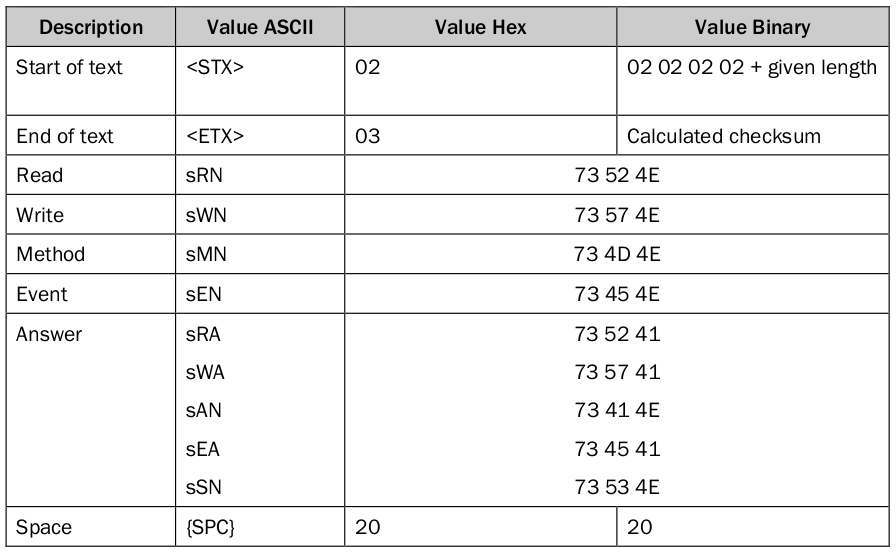
\includegraphics[width=0.5\textwidth]{img/tim55x-telegram-commands.png}
	\caption{Telegram analysieren mit Wireshark}
	\label{fig:tim55x-telegram-commands}
\end{figure}

Um die Kommunikation zwischen Sensor und Applikation zu analysieren wurde mit Wireshark der Netzwerkverkehr aufgezeichnet (Abbildung \ref{fig:tim55x-telegram-wireshark}). Die Anfrage stammt vom SICK eigenen Diagnose-Tool ,,SOPAS Engineering Tool'' und schaltet den Sensor online.
\begin{figure}[H]
	\centering
	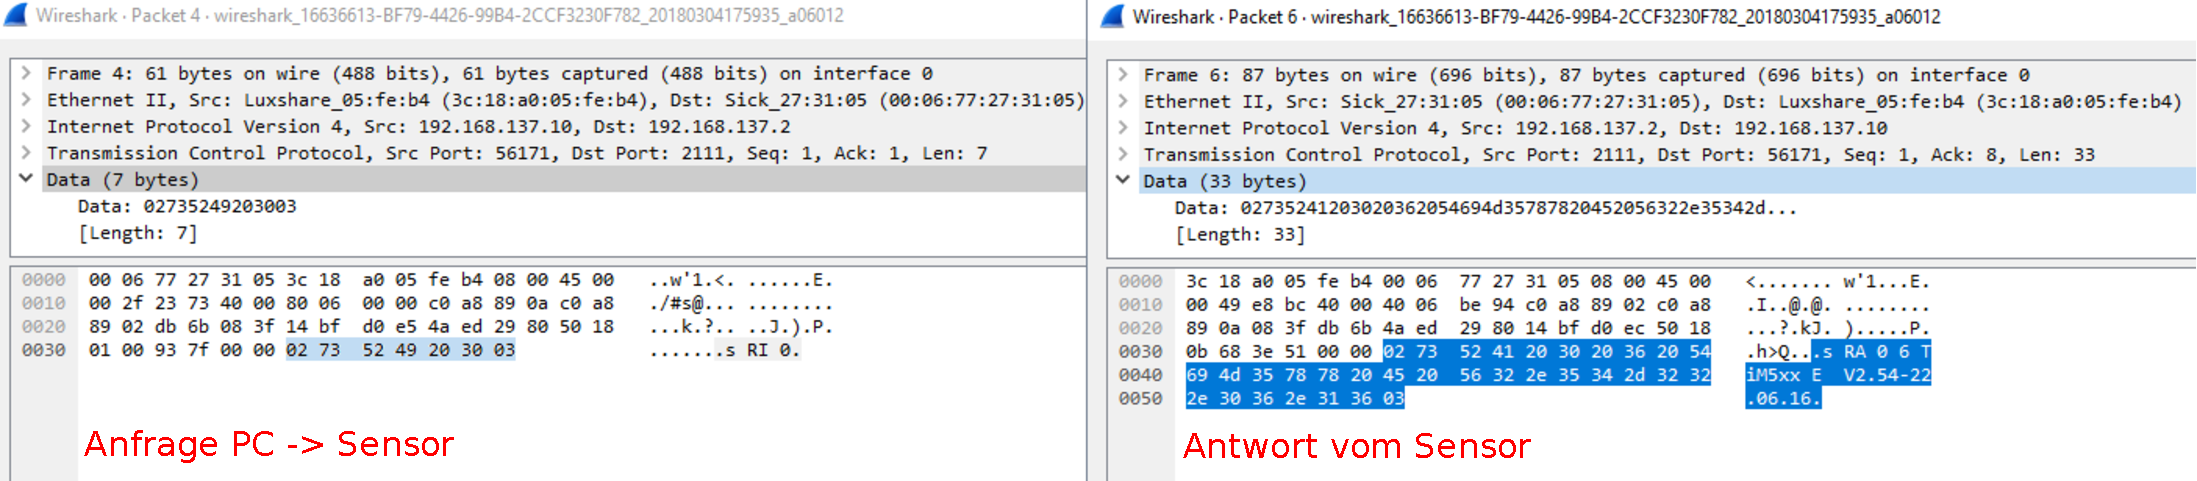
\includegraphics[width=1.0\textwidth]{img/tim55x-telegram-wireshark.pdf}
	\caption{Telegram analysieren mit Wireshark}
	\label{fig:tim55x-telegram-wireshark}
\end{figure}

Die Analyse wurde für alle Aktionen gemacht, welche die von der HFTM zur Verfügung gestellte Library anbietet. Hier eine Zusammenfassung:

\subsubsection{Einzelmessung durchführen (Run single)}
\begin{table}[H]
	\centering
	\begin{tabular}{lp{13cm}} \toprule
		\textbf{Richtung} 	& \textbf{Telegramm-Inhalt}							\\ \midrule
		App -> Sensor		& <STX>sRN LMDscandata<ETX> 							\\ \midrule
		Sensor -> App		& <STX>sRA LMDscandata 1 1 107375C 0 0 2AD8 ... B not defined 0 0 0<ETX>	\\ \bottomrule
	\end{tabular}
	\caption{Kommunikation 'Sensor <--> App' bei Einzelmessung}
	\label{tab:commSingle}
\end{table}

\subsubsection{fortlaufende Messung starten (start)}
\begin{table}[H]
	\centering
	\begin{tabular}{lp{13cm}} \toprule
		\textbf{Richtung} 	& \textbf{Telegramm-Inhalt}							\\ \midrule
		App -> Sensor		& <STX>sEN LMDscandata 1<ETX> 							\\ \midrule
		Sensor -> App		& <STX>sEA LMDscandata 1<ETX>							\\ \midrule
		Sensor -> App (15/s)	& <STX>sSN LMDscandata 1 1 107375C 0 0 E784 ... B not defined 0 0 0<ETX>	\\ \bottomrule
	\end{tabular}
	\caption{Kommunikation 'Sensor <--> App' bei fortlaufender Messung}
	\label{tab:fortlaufendeMessungStart}
\end{table}

\subsubsection{fortlaufende Messung beenden (stop)}
\begin{table}[H]
	\centering
	\begin{tabular}{lp{13cm}} \toprule
		\textbf{Richtung} 	& \textbf{Telegramm-Inhalt}							\\ \midrule
		App -> Sensor		& <STX>sEN LMDscandata 0<ETX> 							\\ \midrule
		Sensor -> App		& <STX>sEA LMDscandata 0<ETX>							\\ \bottomrule
	\end{tabular}
	\caption{Kommunikation 'Sensor <--> App' bei fortlaufender Messung beenden}
	\label{tab:fortlaufendeMessungStop}
\end{table}

\subsection{Implementieren des Mock Services}
Aus diesen Informationen können wir einen simplen Mock-Service implementieren, der lediglich auf diese \underline{drei} Anfragetypen (\ctexttt{sRN LMDscandata}, \ctexttt{sEN LMDscandata 1} und \ctexttt{sEN LMDscandata 0}) von der Applikation hört und jedes mal die gleiche Antwort auf der Anfrage basierend zurück gibt.

\begin{lstlisting}
public class HardwareMock {

    private static ServerSocket serverSocket;
    private static Socket connectionSocket = null;
    private static BufferedReader bufferedReader;
    private static DataOutputStream outputStream;
    private String receivedString = "";

    private final static byte DATA_START = 2;
    private final static byte DATA_END = 3;

    private String singleMeasurementAnswer = "sRA LMDscandata 1 1 107375C 0 0 ...";// nicht komplett
    private String continuousMeasurementAnswer1 = "sEA LMDscandata 1";
    private String continuousMeasurementAnswer2 = "sSN LMDscandata 1 1 107375 ...";// nicht komplett
    private String continuousMeasurementAnswerStop = "sEA LMDscandata 0";

    public HardwareMock (int port, InetAddress bindAddress) throws InterruptedException {
        while (true) {
            try {
                if (serverSocket == null) {
                    LOGGER.info("Opening server socket on '{}:{}'", bindAddress.getHostAddress(), port);
                    serverSocket = new ServerSocket(port, 0, bindAddress);
                }
                if (connectionSocket == null) {
                    LOGGER.info("Start listening for a new connection...");
                    connectionSocket = serverSocket.accept();
                }
                if (bufferedReader == null) {
                    LOGGER.info("Client connected, going on.");
                    bufferedReader = new BufferedReader(new InputStreamReader(connectionSocket.getInputStream()));
                    outputStream = new DataOutputStream(connectionSocket.getOutputStream());
                }
                byte temp = 0;
                while ((temp = (byte) bufferedReader.read()) != -1) {
                    receivedByte(temp);
                    LOGGER.trace("receivedByte ended");
                }
                LOGGER.info("Client disconnected");
                resetSocket();
            } catch (IOException e){
                // ..
            }
        }
    }
}
\end{lstlisting}
Die eigentliche Logik passiert in den Methoden \ctexttt{receivedByte} und \ctexttt{analyseAndPerformAction}. Wir lesen also einfach die Daten auf dem \texttt{InputStream} über den \texttt{BufferedReader} ein und parsen die Bytes sobald wir ein \ctexttt{<ETX>} (end of text) erhalten haben. Danach senden wir sofort beim Erkennen einer bekannten Anfrage (die drei \texttt{if}-Abfragen) die entsprechende Antwort über den \texttt{DataOutputStream} zurück an die Applikation, also dem TiM55x-Service.
\begin{lstlisting}
    public void receivedByte(byte value) {
        LOGGER.trace("receivedByte '{}'", (char)value);
        switch (value){
            case 2:
                this.receivedString = "<STX>";
                LOGGER.info("STX received, clearing String.");
                break;
            case 3:
                this.receivedString = this.receivedString + "<ETX>";
                LOGGER.info("ETX received. String is now: {}", this.receivedString);
                analyseAndPerformAction(this.receivedString);
                break;
            default:
                this.receivedString = this.receivedString + (char)value;
        }
    }

    private void analyseAndPerformAction(String stringToAnalyse){
        if (stringToAnalyse.contains("sRN LMDscandata")) {
            LOGGER.info("Single Scan requested");
            try {
                outputStream.write(DATA_START);
                outputStream.write(singleMeasurementAnswer.getBytes());
                outputStream.write(DATA_END);
                outputStream.flush();
            } catch (IOException e) {
                LOGGER.error("Single Scan error occurred", e);
                return;
            }
         }

         if (stringToAnalyse.contains("sEN LMDscandata 1")) {
             // ..
         }

         if (stringToAnalyse.contains("sEN LMDscandata 0")) {
             // ..
         }

    }
\end{lstlisting}
\chapter{Probleme und Troubleshooting}
\section{GatewayClient Library}

Nach einigen Tests mit der Library GatewayClient gibt es folgende Feststellungen:
\subsection{alle Messages Retained}
Folgendes Listing \ref{lst:retainedMessages} zeigt ein Subscribe-Vorgang mit dem Linux-Client \verb|mosquitto_sub| wenn keine anderen Clients (Abonnenten und Publisher) mit dem MQTT-Broker verbunden sind. Daraus ist ersichtlich, wie alle Messages vom GatewayClient ,,Retained'' publiziert werden. Darum wird beispielsweise der Lidar-service beim Aufstarten gleich den Befehl ,,Einzelmessung starten'' bekommen, in diesem Beispiel sogar mehrfach (Linie 14 und 16):
\begin{lstlisting}[caption={Subscribe mit mosquitto\_sub, Aufstartverhalten},label={lst:retainedMessages}]
$ mosquitto_sub -h localhost -p 1883 -v -t 'Robocup/#' 
Robocup/Lidar/U/192.168.91.2@kicm-fedora.localdomain/S/connection ---
timeStamp: 97641871734173
value: "offline"

Robocup/Lidar/U/192.168.91.2@kicm-fedora.localdomain/S/state ---
- timeStamp: 97642122820521
  state: "INITIALIZING"
- timeStamp: 97642153828641
  state: "STANDBY"

Robocup/Lidar/U/192.168.91.2@kicm-fedora.localdomain/I ---
- timeStamp: 102229304193856
  command: "SINGLE_MEAS"
- timeStamp: 102229322431114       
  command: "SINGLE_MEAS"

Robocup/Lidar/U/192.168.91.2@kicm-fedora.localdomain/E/measurement ---
- timeStamp: 97642626119427
  measurements:
# ... (not complete)

\end{lstlisting}

\chapter{Ausblick}
\section{API / Bindings in seprartem Projekt}
\label{sec:separatebindings}
Beim TiM55x-Service habe ich unbewusst die HFTM-\acrshort{lidar}-Library bis zum Contract durchdrücken lassen. Dies habe ich exemplarisch so beibehalten. Das Problem ist folgendes: der Servant, der mit diesen Service kommuniziert, braucht alle Objekte vom Contract. Die Dependencies eines Services werden beim standardmässigen bauen eines Jars aber nicht eingepackt. Für die Ausführung des Services mit dem Befehl \ctexttt{java -jar paketname.jar} packen wir aber sowieso alle Dependecies in ein Jar, damit lediglich diese Datei aufs Zielsystem deployed / kopiert werden muss. Der Grössenunterschied ist allerdings immens und deshlab sollte ein Servant nicht dieses so genannte Fat-Jar als Depedency reinziehen.

TODO

\begin{itemize}
	\item
	GatewayClient und API an MQTT trennen
	
	\item
	MQTT API versionieren -> 'alte Dependencies' funktionieren weiterhin mit dem 'alten Service'
\end{itemize}

\section{Fehlerbehandlung innerhalb der Services}
TODO

\section{Servant abkürzen}
TODO
Während intensiven Diskussionen mit Reto zum Thema wie sich der Datenaustausch von Service zu Service abkürzen lässt, ist folgende Idee zu Stande gekommen:

\section{Performance Serialisieren / Deserialisieren}
TODO

\chapter{Projektmanagement}
\section{Vorarbeiten}
Diese Bachelorarbeit basiert nicht auf einer Projekt2-Arbeit. Die Bachelorarbeit entsteht also während einem Semester.

\section{Aufgabenstellung}
\label{sec:aufgabenstellung-messbar}
TODO:
konkrete Aufgabenstellung, was soll raus kommen -> Howto für Studenten der \acrshort{hftm}

\section{Rahmenbedingungen}
Die Rahmenbedingungen dieses Projektes wurden gemeinsam mit dem Betreuer definiert:
\begin{itemize}
	\item Source-Code für \acrshort{lidar}-Ansteuerung von \acrshort{hftm}, verwenden als Library
	\item Library \verb|ch.quantasy.mqtt.gateway|\cite{ch.quantasy.mqtt.gateway} von Reto Koenig als Schnittstelle zwischen Hardware, User und Event-Bus
\end{itemize}

\section{Projektplan und Meilensteine}
TODO
\subsection{fixe Termine}
\begin{table}[H]
	\centering
	\begin{tabular}{lll} \toprule
		\textbf{Datum} 			& \textbf{Termin Beschreibung}		& \textbf{Bemerkungen}		\\ \midrule
		Fr., 01.06.2018, 12:00		& Poster für Ausstellung 		& E-Mail an Heinz.Kipfer@bfh.ch	\\ \midrule
		Mo., 04.06.2018 		& Book - Freigabe Inhalte		& https://students.book.bfh.ch	\\ \midrule
		Mo., 11.06.2018 		& Book - Freigabe Layout		& https://students.book.bfh.ch	\\ \midrule
		Do., 14.06.2018, 20:00		& Abgabe Bericht			&  				\\ \midrule
		Fr., 15.06.2018, 10:40 - 10:55	& Präsentation Arbeit (Finaltag)	&  				\\ \midrule
		Fr., 22.06.2018			& Abgabe Film				& hochladen in Moodle		\\ \midrule
		Mi., 27.06.2018, 10:00 - 12:00	& Verteidigung				&				\\ \bottomrule
	\end{tabular}
	\caption{fixe Termine während der Bachelorarbeit}
	\label{tab:fixeTermine}
\end{table}


\section{Meetings}
Mit dem Betreuer wurden zu Beginn dieser Arbeit die Meetings auf jede zweite Woche festgelegt. Bei Bedarf können Meetings auch Adhoc stattfinden.
\subsection{Protokolle}
\subsubsection{Startvorlesung mit Herr Anrig (Mo., 19.02.2018)}
\begin{itemize}
	\item Aufgabenstellung erhalten
	\item Termine allgemein, alles auf Moodle
	\item Video ab diesem Semester Pflicht
	\item Eintrag im Book, Termin folgt
	\item Plakat Vorlagen etc., Termin folgt
\end{itemize}

\subsubsection{Treffen mit Reto (Fr., 23.02.2018)}
\begin{itemize}
	\item Code für Java-GUI Software erhalten (Zip, Mail) -> Pushed auf https://gitlab.ti.bfh.ch/kilcm1/hftm-lidar
	\item Einführung in die Github Repos von knr1 (Reto Koenig) -> https://github.com/knr1?tab=repositories
	\item Festlegung der Treffen: alle zwei Wochen in Biel
\end{itemize}
Ziele: Lernbuch für HFTM (entweder in Doku integriert oder extern)


\subsubsection{Treffen mit Reto (Do., 08.03.2018)}
Erste Schritte mit dem GatewayClient gezeigt (LidarService). Weitere Schritte:
\begin{itemize}
	\item Servant und kleiner UI-Service (console writer) implementieren
	\item Danach Dokumentieren der ersten Erkenntnisse
	\item Vorschlag für Treffen mit Experten (Dr. Joachim Wolfgang Kaltz)
\end{itemize}
\subsubsection{Treffen mit Experte (Mo., 19.03.2018)}
\begin{itemize}
	\item Vorhaben erklärt, HFTM und Studenten erläutert
	\item Experte ist einverstanden: die Arbeit könne gut ein Handbuch für die Studenten der HFTM sein. Kein Problem.
	\item Referenz-Setup mit den zwei Services und dem Servant gezeigt (Lidar, Console Client, Servant)
\end{itemize}
Weitere Schritte: Weiteres Meeting mit Experte, Alain und Reto Mitte Mai.
\subsubsection{Treffen mit Reto (Do., 22.03.2018)}
nächste Schritte: Doku

\subsubsection{Treffen mit Reto und Alain (Do., 13.04.2018)}
\begin{itemize}
	\item Zugriff auf aktuellen Sourcecode vom Roboter erhalten (auf gitlab.com \cite{gitlab.com/solidus/hefei})
	\item Niveau ist nicht sehr hoch, darf die Studenten nicht gleich überfordern. Java wird in 34 Lektionen vor dem Arbeiten am Robocup erst ausgebildet. Vorher haben die Meisten noch nie objektorientiert programmiert.
	\item Robi hat Intel i5-Basierter PC drauf (also doch kein Raspi) = ebenbürdig mit meinem Lenovo Yoga 2 Pro
\end{itemize}

\subsubsection{Treffen mit Reto (Do., 26.04.2018)}
\begin{itemize}
	\item Alternativen mit "Kein Gluelayer"/Servant innerhalb einer Domain ansprechen, aber weiter wie bisher: zwischen jedem Service gibt es den Servant.
	\item Wenn es im Servant zu Ressourcen-Problemen kommt, verwenden wir eine andere Struktur als YAML/JSON (Bsp. Google's Protocol buffers)
	\item nächste Schritte: Doku, Linien-Finder anschauen, Testing
\end{itemize}

\subsubsection{Treffen mit Reto (Do., 03.05.2018)}
\begin{itemize}
	\item Idee Services über Reference zusammenhängen, ohne die Daten durch den Servant zu schleusen, wenn kompatibel. Der Servant würde den entsprechenden Services das mitteilen.
	\item Zerreissen der "Library" für EdgeDetection, da Refactoring notwendig (Bsp. Naming der Koordinatensysteme Polar und Kartesisch)
\end{itemize}

\subsubsection{Treffen mit Reto (Do., 17.05.2018)}
\begin{itemize}
	\item Architekturbild (Datenfluss löschen und beim anderen Architekturbild bleiben)
	\item erklären weshalb nur der letzte LidarIntent genommen wird
	\item zwei Dokument-"Parts": transition und setup (erklären weshalb)
	\item pushen vom EdgeDetector - Stand heute
	\item Adapter auf Service ändern
	\item Annotations einführen für Contract
	\item Umbenennung: Lidar-Service heisst TIM55x und EdgeDetector heisst 2DEdgeDetector
\end{itemize}



\subsection{abgesagte Meetings}
\subsubsection{Treffen mit Reto und Alain (Do., 05.04.2018)}
abgesagt da Reto krank -> verschoben auf Fr., 13.04.2018, 09:00

\subsubsection{Treffen mit Reto (Do., 19.04.2018)}
abgesagt da Reto krank -> verschoben auf Do., 26.04.2018, 15:30

\section{Journal}
TODO: Bild vom Excel einfügen am Schluss
%---------------------------------------------------------------------------

% Attachment:
%---------------------------------------------------------------------------
\appendix
\settocdepth{section}
\chapter{Anhang}
\pagenumbering{roman}
\section{Selbstständigkeitserklärung}
\section{Anderes}


%---------------------------------------------------------------------------



%---------------------------------------------------------------------------

% Glossary
%---------------------------------------------------------------------------
%\cleardoublepage
%\phantomsection 
%\addcontentsline{toc}{chapter}{Glossar}
%\renewcommand{\glossaryname}{Glossar}
%\printglossary

% Glossar ausgeben
\printglossary[title=Glossar]
\pagenumbering{Roman}

% Abkuerzungen ausgeben
\printglossary[type=\acronymtype, title=Abkürzungsverzeichnis]
%---------------------------------------------------------------------------

% Bibliography
%---------------------------------------------------------------------------
%\cleardoublepage
%\phantomsection 
%\addcontentsline{toc}{chapter}{Literaturverzeichnis}
%\bibliographystyle{IEEEtran}
%\bibliography{datenbanken/bibliography}{}
\printbibliography[title={Literaturverzeichnis},heading=bibintoc]

%---------------------------------------------------------------------------

% Listings
%---------------------------------------------------------------------------
%\cleardoublepage
%\phantomsection 
\addcontentsline{toc}{chapter}{Abbildungsverzeichnis}
\listoffigures
%\cleardoublepage
%\phantomsection 
\addcontentsline{toc}{chapter}{Tabellenverzeichnis}
\listoftables
%---------------------------------------------------------------------------

% Index
%---------------------------------------------------------------------------
%\cleardoublepage
%\phantomsection 
%\addcontentsline{toc}{chapter}{Stichwortverzeichnis}
%\renewcommand{\indexname}{Stichwortverzeichnis}
%\printindex
% Usage:
% Hello World\index{Hello World}
%---------------------------------------------------------------------------

% Selbständigkeitserklärung
%---------------------------------------------------------------------------
%\cleardoublepage
%\phantomsection 
\addcontentsline{toc}{chapter}{Selbständigkeitserklärung}
\chapter*{Selbständigkeitserklärung}
\label{chap:selbstaendigkeitserklaerung}

\vspace*{10mm} 

Ich/wir bestätige/n, dass ich/wir die vorliegende Arbeit selbstständig und ohne Benutzung anderer als der im Literaturverzeichnis angegebenen Quellen und Hilfsmittel angefertigt habe/n. Sämtliche Textstellen, die nicht von mir/uns stammen, sind als Zitate gekennzeichnet und mit dem genauen Hinweis auf ihre Herkunft versehen. 

\vspace{15mm}

\begin{tabbing}
xxxxxxxxxxxxxxxxxxxxxxxxx\=xxxxxxxxxxxxxxxxxxxxxxxxxxxxxx\=xxxxxxxxxxxxxxxxxxxxxxxxxxxxxx\kill
Ort, Datum:		\> [Biel/Burgdorf], \versiondate \\ \\ 
Namen Vornamen:	\> [Test Peter] 	\> [Müster Rösä] \\ \\ \\ \\ 
Unterschriften:	\> ......................................\> ...................................... \\
\end{tabbing}


%---------------------------------------------------------------------------
\end{document}
